\documentclass[11pt]{article}

\usepackage[utf8]{inputenc}
\usepackage[T1]{fontenc}
\usepackage[french]{babel}
\usepackage{lmodern}
\usepackage{geometry}
\usepackage{setspace}
\usepackage{graphicx}
\usepackage{titlesec}
\usepackage{enumitem}
\usepackage{hyperref}
\usepackage{fancyhdr}
\usepackage{amsmath}
\usepackage{amssymb}
\usepackage{tikz}
\usepackage{algorithm}
\usepackage{algpseudocode}
\usepackage{float}
\usepackage{booktabs}

\usetikzlibrary{arrows.meta,positioning}
\usetikzlibrary{arrows.meta,positioning,calc}

\geometry{margin=2.5cm}
\setlength{\parindent}{0pt}
\setlength{\parskip}{0.4em}
\onehalfspacing

% Simple page numbering at the bottom of the page
\pagestyle{fancy}
\fancyhf{}
\fancyfoot[C]{\thepage}
\renewcommand{\headrulewidth}{0pt}

\begin{document}


\begin{titlepage}

    \noindent
    \begin{minipage}{0.5\textwidth}
        
\includegraphics[width=4cm]{Logo/Paris1logo.png}
    \end{minipage}
    \begin{minipage}{0.5\textwidth}
        \raggedleft
        
\includegraphics[width=4cm]{Logo/SAMMlogo.png}
    \end{minipage}

    \vspace{6cm}

    \begin{center}

        {\huge \textbf{Hidden Markov Models and Application to the VIX}}\\[1.2cm]

        {\large Under the supervision of \textit{Joseph Rynkiewicz and Jean-Marc Bardet.}}\\[0.8cm]

        {\large By Marius Requillart and Maxime Delpech.}\\[0.8cm]

        {\large 2026}
    \end{center}

    \vspace{1cm} 
    \begin{center} 
        \begin{minipage}{0.88\textwidth} 
            \begin{center} {\large \textbf{Abstract}} 
            \end{center} 
            \vspace{0.3cm} 
            \small This work studies hidden Markov models as a tool for modelling financial time series subject to regime changes. After presenting the probabilistic framework of HMMs, we detail the main inference and estimation algorithms: Forward for likelihood computation, Viterbi for decoding hidden states, and Baum--Welch for parameter estimation. These methods are first evaluated on simulated data, which makes it possible to compare the estimated regimes and parameters with the true values. They are then applied to the VIX index in order to identify different volatility regimes and analyse their stability as well as the predictive quality of the model. This study thus illustrates the relevance of HMMs for representing and interpreting the latent dynamics of financial markets. 
            \vspace{0.4cm} 
        \end{minipage} 
    \end{center}

    \vfill
\end{titlepage}

\setcounter{page}{1}

% Table of contents

\vspace{1cm}

\thispagestyle{fancy}

\begin{center}
    {\LARGE \textbf{TABLE OF CONTENTS}}
\end{center}

\vspace{0.5cm}

\tableofcontents

\newpage


\newpage
%%%%%%%%%%%%%%%%
% Beginning of the project
%%%%%%%%%%%%%%%%

\section{Introduction}


Financial time series play a central role in quantitative finance, as they make it possible to analyse the evolution of asset prices, returns, volatility, and trading volumes over time. However, these series often exhibit complex behaviour: they are noisy, irregular, sometimes unstable, and may be characterised by sudden changes in dynamics. A single financial series may thus alternate between relatively calm periods and periods of high uncertainty, which makes its analysis particularly challenging.

Hidden Markov Models constitute a suitable probabilistic framework for modelling this type of phenomenon. Their principle is based on the existence of a latent state, which is not directly observable and evolves over time according to a Markov chain. The available observations, such as financial returns, are then assumed to depend on this hidden state. 

The interest of these models lies in their ability to reveal a hidden structure underlying the observed data. They make it possible not only to detect regime changes, but also to provide an economic and financial interpretation of the results obtained. The identified hidden states may, for example, be associated with phases of growth, financial stress, high uncertainty, or a return to a more stable situation. Thus, the analysis is not limited to a statistical classification of the observations: it may also help relate the detected regimes to market events, changes in expectations, or variations in the level of risk.

In this work, we study hidden Markov models and their applications to financial time series. We first present the theoretical framework of these models, before addressing the main inference and estimation algorithms, in particular the Viterbi and Baum--Welch algorithms. We then analyse their use for identifying different market regimes and gaining a better understanding of the evolution of financial series.

\newpage

\section{Definition and Properties of Hidden Markov Models}
%%%%%%%%%%%%%%
% Beginning of Section 2.2 
%%%%%%%%%%%%%%

\subsection{Definition of a Hidden Markov Model}

Hidden Markov Models (HMMs) are statistical models used in situations where latent states are not directly observable. The observable data are generated by these states according to a conditional probability distribution.

\subsubsection{Observable and Hidden Random Variables}

\textbf{Definition.} 
The hidden states are modelled by a Markov process $(X_t)_{t \in \mathbb{N}}$ taking values in a finite set $E  = \{1,\dots,N\}$. 
We denote by $A = (a_{ij})$ the transition matrix defined by:
\[
a_{ij} = \mathbb{P}(X_{t+1} = j \mid X_t = i).
\]

\vspace{0.3cm}

\textbf{Definition.} 
The observations are modelled by a process $(Y_t)_{t \in \mathbb{N}}$ taking values in a set $O$. 
Conditionally on the hidden states, the variables $(Y_t)$ are independent and satisfy:
\[
\mathbb{P}(Y_t = y \mid X_t = i) = b_i(y),
\]
where $B = (b_i(y))$ is the emission matrix (or family).

\vspace{0.3cm}

\textbf{Definition.} 
A hidden Markov model is defined by the triplet $(A, B, \pi)$ where:
\begin{itemize}
    \item $A$ is the transition matrix of the hidden states,
    \item $B$ is the emission distribution of the observations,
    \item $\pi$ is the initial distribution, with $\pi_i = \mathbb{P}(X_1 = i)$.
\end{itemize}
\vspace{0.3cm}

\subsubsection{Joint Distributions and Likelihood}

\textbf{Property:}
Let $X$ = ($X_1$, \dots, $X_T$) be the sequence of hidden states and $Y$ = ($Y_1$, \dots, $Y_T$) the sequence of observations. The distribution of the observations conditionally on the sequence of hidden states is: 
\[
\mathbb{P}(Y \mid X) = \prod_{t=1}^T \mathbb{P}(Y_t \mid X_t) 
\]

\textbf{Proof:}
\[
\mathbb{P}(Y \mid X) = \prod_{t=1}^T \mathbb{P}(Y_t \mid X_1, \dots X_T,Y_1, \dots Y_{t-1})=\prod_{t=1}^T \mathbb{P}(Y_t \mid X_t)  
\]
\vspace{0.3cm}

\textbf{Property:}
Let $X$ = ($X_1$, \dots, $X_T$) be the sequence of hidden states and $Y$ = ($Y_1$, \dots, $Y_T$) the sequence of observations. The joint distribution of the observations and hidden states is given by: 
\[
\mathbb{P}(Y, X) = \pi_{X_1} \prod_{t=2}^T \mathbb{P}(X_{t} \mid X_{t-1}) \prod_{t=1}^T \mathbb{P}(Y_t \mid X_t)
\]

\textbf{Proof:}
\begin{align*}
\mathbb{P}(X, Y) 
&= \mathbb{P}(X_1, Y_1) \prod_{t=2}^T \mathbb{P}(X_t,Y_t \mid X_1, \dots, X_{t-1}, Y_1,\dots, Y_{t-2}) \\
&= \mathbb{P}(X_1)\mathbb{P}(Y_1 \mid X_1) 
\prod_{t=2}^T \mathbb{P}(X_t \mid X_1, \dots, X_{t-1}, Y_1,\dots, Y_{t-2})
\mathbb{P}(Y_t \mid X_1, \dots, X_{t-1}, Y_1,\dots, Y_{t-2}) \\
&= \mathbb{P}(X_1)\mathbb{P}(Y_1 \mid X_1) 
\prod_{t=2}^T \mathbb{P}(X_t \mid X_{t-1}) \mathbb{P}(Y_t \mid X_t) \\
&= \mathbb{P}(X_1) \prod_{t=2}^T \mathbb{P}(X_t \mid X_{t-1}) \prod_{t=1}^T \mathbb{P}(Y_t \mid X_t) \\
&= \pi_{X_1} \prod_{t=2}^T \mathbb{P}(X_t \mid X_{t-1}) \prod_{t=1}^T \mathbb{P}(Y_t \mid X_t)
\end{align*}
\vspace{0.3cm}

\textbf{Remark:}
The distribution of the observations at each time $t$ depends on the hidden state at that time and not on the previous states. 
\vspace{0.3cm}

\textbf{Example:}
Consider a hidden Markov model with two states $A$ and $B$. 
Assuming that the observations are Gaussian conditionally on the hidden state, we have:
\[
\mathcal{L}(Y_t | {X_t=A}) \sim \mathcal{N}(\mu_{A}, \sigma^2_{A})
\]
\[
\mathcal{L}(Y_t | {X_t=B}) \sim \mathcal{N}(\mu_{B}, \sigma^2_{B})
\]
\vspace{0.3cm}

\textbf{Remark:}
$X_t$ acts as a distribution selector for $Y_t$.
\vspace{0.3cm}

\subsubsection{General Example of a Hidden Markov Model}

Consider a simple example of a hidden Markov model with two states $C$ and $V$ (for "calm" and "volatile") and Gaussian observations conditional on these states.\\
Let $E = \{C, V\}$ be the state space, and let $\pi$ denote the initial distribution, for example $\pi_0 = (0.5, 0.5)$, indicating that the process starts with equal probability in states $C$ and $V$.\\
The transition matrix $A$ may be defined as follows:
\[
A =
\begin{pmatrix}
0.9 & 0.1 \\
0.2 & 0.8
\end{pmatrix}
\]
with $a_{ij} = \mathbb{P}(X_{t+1} = j \mid X_t = i)$.

\vspace{0.3cm}

The family of parametric densities $B$ may be defined by the Gaussian distributions conditional on each state:
\[
B =
\begin{cases}
\mathcal{L}(Y_t \mid X_t = C) \sim \mathcal{N}(\mu_C, \sigma_C^2) \\
\mathcal{L}(Y_t \mid X_t = V) \sim \mathcal{N}(\mu_V, \sigma_V^2)
\end{cases}
\]

\vspace{0.5cm}
\textbf{Note:}
The transition matrix $A$ is not known in most applications; it must be estimated from the observation data, for example using the Baum--Welch algorithm, which we will study later.
\vspace{1.5cm}

\begin{figure}[h]
\centering
\begin{tikzpicture}[
    node distance=2cm,
    every node/.style={draw, circle, minimum size=1cm},
    arrow/.style={->, thick}
]

% Hidden states
\node (X1) {$X_t$};
\node (X2) [right=of X1] {$X_{t+1}$};

% Observations
\node (Y1) [below=of X1] {$Y_t$};
\node (Y2) [below=of X2] {$Y_{t+1}$};

% Transitions
\draw[arrow] (X1) -- node[midway, above, draw=none] {$a_{ij}$} (X2);

% Emissions
\draw[arrow] (X1) -- 
node[midway, left, draw=none] {$\mathbb{P}(Y_t \mid X_t)$} 
(Y1);

\draw[arrow] (X2) -- 
node[midway, right, draw=none] {$\mathbb{P}(Y_{t+1} \mid X_{t+1})$} 
(Y2);

\end{tikzpicture}
\caption{Hidden Markov Model (HMM)}
\end{figure}


\newpage



\subsubsection{Remarks on the Observations}

\textbf{Property:}
The total probability of the observations $(Y_t)_{t}$ is given by: 
\[
\mathbb{P}(Y) = \sum_{X}\mathbb{P}(Y,X) = \sum_{}\mathbb{P}(Y \mid X)\mathbb{P}(X)
\]
\vspace{0.3cm}

\textbf{Property:}
In a non-degenerate HMM, the observation process $(Y_t)_{t}$ is not a Markov process, even though the hidden states $(X_t)_{t}$ are. 

\textbf{Proof:}

If the observation process $(Y_t)_{t}$ were Markovian, then we would have
\[
\mathbb{P}(Y_{n+1} \mid Y_1,\dots,Y_n) = \mathbb{P}(Y_{n+1} \mid Y_n).
\]

However, for $K$ hidden states, we have
\begin{align*}
\mathbb{P}(Y_{n+1} \mid Y_1,\dots,Y_n)
&= \sum_{i=1}^{K} \mathbb{P}(Y_{n+1}, X_{n+1}=i \mid Y_1,\dots,Y_n) \\
&= \sum_{i=1}^{K} \mathbb{P}(Y_{n+1} \mid X_{n+1}=i, Y_1,\dots,Y_n)\,
\mathbb{P}(X_{n+1}=i \mid Y_1,\dots,Y_n) \\
&= \sum_{i=1}^{K} \mathbb{P}(Y_{n+1} \mid X_{n+1}=i)\,
\mathbb{P}(X_{n+1}=i \mid Y_1,\dots,Y_n).
\end{align*}

Moreover, 
\begin{align*}
\mathbb{P}(X_{n+1}=i \mid Y_1,\dots,Y_n)
&= \sum_{j=1}^{K} \mathbb{P}(X_{n+1}=i, X_{n}=j \mid Y_1,\dots,Y_n) \\
&= \sum_{j=1}^{K} \mathbb{P}(X_{n+1}=i \mid X_{n}=j, Y_1,\dots,Y_n) \mathbb{P}(X_{n}=j \mid Y_1, \dots Y_n)\\
&= \sum_{j=1}^{K} \mathbb{P}(X_{n+1}=i \mid X_{n}=j) \mathbb{P}(X_n=j \mid Y_1, \dots Y_n)\\
&= \sum_{j=1}^{K} a_{ji} \mathbb{P}(X_n=j \mid Y_1, \dots Y_n).
\end{align*}

and, 
\begin{align*}
\mathbb{P}(X_{n}=j \mid Y_1,\dots,Y_n) 
&= \mathbb{P}(X_n=j, Y_1 \dots Y_n) / \mathbb{P}(Y_1 \dots Y_n) \\[0.3cm]
&= \frac{\mathbb{P}(Y_n \mid X_n=j,Y_1 \dots Y_{n-1}) \mathbb{P}(X_n=j, Y_1 \dots Y_{n-1})}{\mathbb{P}(Y_1 \dots Y_n)} \\[0.3cm]
&= \frac{\mathbb{P}(Y_n \mid X_n=j) \mathbb{P}(X_n=j \mid Y_1 \dots Y_{n-1}) \mathbb{P}(Y_1 \dots Y_{n-1})}{\mathbb{P}(Y_n \mid Y_1 \dots Y_{n-1}) \mathbb{P}(Y_1 \dots Y_{n-1})}\\[0.3cm]
&= \frac{\mathbb{P}(Y_n \mid X_n=j) \mathbb{P}(X_n=j \mid Y_1 \dots Y_{n-1})}{\mathbb{P}(Y_n \mid Y_1 \dots Y_{n-1})}.
\end{align*}

We therefore have: 
\[
\mathbb{P}(Y_{n+1}\mid Y_1 \dots Y_n ) = \sum_{i=1}^{K} \sum_{j=1}^K a_{ji} \frac{\mathbb{P}(Y_{n+1} \mid X_{n+1} = i) \mathbb{P}(Y_n \mid X_n=j) \mathbb{P}(X_n=j \mid Y_1 \dots Y_{n-1})}{\mathbb{P}(Y_n \mid Y_1 \dots Y_{n-1})}.
\]

The same procedure is used to compute $\mathbb{P}(X_n = j \mid Y_1 \dots Y_{n-1})$, which reduces the dependence to $Y_{n-1}$. This recursive procedure is continued until the term depending on $Y_1$ is reached.

Thus, the term
\[
\mathbb{P}(X_{n+1}=i \mid Y_1,\dots,Y_n)
\]
generally depends on the entire observed past $(Y_1,\dots,Y_n)$, and not only on $Y_n$.

Therefore, in general,
\[
\mathbb{P}(Y_{n+1} \mid Y_1,\dots,Y_n) \neq \mathbb{P}(Y_{n+1} \mid Y_n),
\]
which shows that the observation process $(Y_t)$ is not Markovian.

\newpage

\section{Three Main Problems in HMMs}

%%%%%%%%%%%%%%%%%%
%% Beginning of Part 3 on algorithms
%%%%%%%%%%%%%%%%%%

\subsection{Likelihood Estimation and the Forward Algorithm}

\textbf{Problem:}
How can the likelihood $\mathbb{P}(Y)$ of an observation sequence $Y$ under an HMM $(A, B, \pi)$ be computed efficiently? \\ 

We assume that the transition matrix $A$, the emission matrix $B$, and the initial distribution $\pi$ are known. \\ 

We know that the likelihood of $Y$ is given by:
\[
\mathbb{P}(Y) = \sum_{X}\mathbb{P}(Y,X) = \sum_{X}\mathbb{P}(Y \mid X)\mathbb{P}(X).
\]
However, for $N$ hidden states and an observation sequence of length $T$, the number of possible hidden sequences is $N^T$, which makes direct computation exponentially complex if carried out naively. \\ 
The optimal solution is to use the Forward algorithm, which computes $\mathbb{P}(Y)$ with complexity $O(N^2T)$. \\ 

This algorithm is based on dynamic programming and uses an intermediate variable $\alpha_t(i)$ representing the probability of observing the sequence $y_1 \dots y_t$ and being in hidden state $i$ at time $t$.\\
Formally, $\alpha_t(i)$ is defined as: 
\[
\alpha_t(i) = \mathbb{P}(y_1, \dots, y_t, X_t = i).
\]

\vspace{0.5cm}
\begin{algorithm}[H]
\caption{Forward Algorithm}
\label{alg:forward}
\begin{algorithmic}[1]
\Require Transition matrix $A = (a_{ij})_{1 \leq i,j \leq N}$,
emission probabilities $B = (b_i(y))_{1 \leq i \leq N}$,
initial distribution $\pi = (\pi_i)_{1 \leq i \leq N}$,
observation sequence $Y = (y_1,\dots,y_T)$
\Ensure Likelihood $\mathbb{P}(Y)$

\Statex
\Statex \textbf{Initialisation}
\For{$i = 1,\dots,N$}
    \State $\alpha_1(i) \gets \pi_i b_i(y_1)$
\EndFor

\Statex
\Statex \textbf{Recursion}
\For{$t = 2,\dots,T$}
    \For{$j = 1,\dots,N$}
        \State $\displaystyle \alpha_t(j) \gets b_j(y_t)
        \sum_{i=1}^N \alpha_{t-1}(i)a_{ij}$
    \EndFor
\EndFor

\Statex
\Statex \textbf{Termination}
\State $\displaystyle \mathbb{P}(Y) \gets \sum_{i=1}^N \alpha_T(i)$
\State \Return $\mathbb{P}(Y)$

\end{algorithmic}
\end{algorithm}

where $a_{ij}$ is the transition probability from state $i$ to state $j$, $b_j(y_{t})$ is the probability of observing $Y_t = y_t$ conditionally on being in state $j$ at time $t$, and $\pi_i$ is the initial probability of being in state $i$.

The Forward algorithm thus computes the likelihood of a given observation sequence efficiently, while avoiding the direct computation of all possible hidden-state sequences.
\vspace{0.5cm}

\textbf{Complexity analysis:}\\
During initialisation, $N$ operations of complexity $O(1)$ are performed to compute $\alpha_1(i)$ for $i=1, \dots, N$, giving a complexity of $O(N)$.\\
During recursion, for each time $t$ from 2 to $T$, $N$ operations are performed to compute $\alpha_t(j)$ for $j=1, \dots, N$. Each computation of $\alpha_t(j)$ requires a sum of $N$ terms, corresponding to a complexity of $O(N^2)$ at each time $t$. Thus, the total complexity of the recursion is $O(N^2T)$.\\
At termination, a sum of $N$ terms is performed to compute $\mathbb{P}(Y)$, corresponding to a complexity of $O(N)$.\\
Combining these different steps gives a total algorithmic complexity of $O(N^2T)$, which is much more efficient than the exponential complexity $O(N^T)$ of direct computation. 

\vspace{0.5cm}

For clarity, the Forward algorithm may be represented in trellis form: 

\begin{figure}[H]
\centering
\resizebox{\textwidth}{!}{%
\begin{tikzpicture}[
    >=Stealth,
    etat/.style={
        circle,
        draw,
        minimum size=1.05cm,
        inner sep=0pt,
        font=\large
    },
    init/.style={
        circle,
        draw,
        minimum size=0.95cm,
        inner sep=0pt,
        font=\large
    },
    fleche/.style={
        ->,
        line width=0.6pt,
        shorten >=1pt,
        shorten <=1pt
    },
    formule/.style={
        font=\small
    },
    contrib/.style={
        font=\scriptsize,
        fill=white,
        inner sep=1pt
    }
]

% Initial node
\node[init] (pi) at (0.6,0) {$\pi$};

% Hidden states
\node[etat] (e21) at (4.2,1.15) {$e_2$};
\node[etat] (e11) at (4.2,-1.15) {$e_1$};

\node[etat] (e22) at (11.2,1.15) {$e_2$};
\node[etat] (e12) at (11.2,-1.15) {$e_1$};

\node[etat] (e23) at (18.2,1.15) {$e_2$};
\node[etat] (e13) at (18.2,-1.15) {$e_1$};

% Observations
\node at (4.2,-2.45) {$y_1$};
\node at (11.2,-2.45) {$y_2$};
\node at (18.2,-2.45) {$y_3$};

% Initial transitions
\draw[fleche] (pi) -- node[above left, contrib] {$\pi_2 b_2(y_1)$} (e21);
\draw[fleche] (pi) -- node[below left, contrib] {$\pi_1 b_1(y_1)$} (e11);

% Transitions between t=1 and t=2
\draw[fleche] (e21) -- node[above, contrib] {$\alpha_1(2)a_{22}b_2(y_2)$} (e22);
\draw[fleche] (e21) -- node[pos=0.28, below, sloped, contrib] {$\alpha_1(2)a_{21}b_1(y_2)$} (e12);
\draw[fleche] (e11) -- node[pos=0.72, above, sloped, contrib] {$\alpha_1(1)a_{12}b_2(y_2)$} (e22);
\draw[fleche] (e11) -- node[below, contrib] {$\alpha_1(1)a_{11}b_1(y_2)$} (e12);

% Transitions between t=2 and t=3
\draw[fleche] (e22) -- node[above, contrib] {$\alpha_2(2)a_{22}b_2(y_3)$} (e23);
\draw[fleche] (e22) -- node[pos=0.28, below, sloped, contrib] {$\alpha_2(2)a_{21}b_1(y_3)$} (e13);
\draw[fleche] (e12) -- node[pos=0.72, above, sloped, contrib] {$\alpha_2(1)a_{12}b_2(y_3)$} (e23);
\draw[fleche] (e12) -- node[below, contrib] {$\alpha_2(1)a_{11}b_1(y_3)$} (e13);

% Column headings
\node at (4.2,2.05) {\(\alpha_1(i)\)};
\node at (11.2,2.05) {\(\alpha_2(j)\)};
\node at (18.2,2.05) {\(\alpha_3(j)\)};

% Recurrence formula
\node[formule, align=center] at (11.2,2.85)
{\(\displaystyle
\alpha_t(j)=b_j(y_t)\sum_{i=1}^{N}\alpha_{t-1}(i)a_{ij}
\)};

% Time labels
\node at (4.2,-3.05) {\(t=1\)};
\node at (11.2,-3.05) {\(t=2\)};
\node at (18.2,-3.05) {\(t=3\)};

% Likelihood finale
\node[formule, align=center] at (11.2,-3.75)
{\(\displaystyle L=\sum_{i=1}^{N}\alpha_T(i)\)};

\end{tikzpicture}
}
\vspace{0.35cm}
\caption{Trellis of the Forward Algorithm}
\label{fig:treillis-forward}
\end{figure}


\subsection{Decoding and the Viterbi Algorithm}

Consider a new problem: decoding a state sequence from a series of observations $Y_1,\dots,Y_T$.
We aim to recover the hidden component of the model.\\
i.e. to recover a posteriori the ``true'' state sequence $X = (X_1, \dots, X_T)$ that occurred to generate a series of observations, given the initial distribution, transition matrix, and emission probabilities.

It is clear that there is not always a ``true'' state sequence; we must therefore introduce optimality criteria to address our problem.

A first approach, which could be described as ``greedy'', would be to choose, at each time $t$, the state $X_t$ for which the probability of observing $Y_t$ is largest.
This optimality criterion maximises the expected number of states correctly decoded individually.

However, this may lead to several problems with the resulting state sequence. Since the local criterion ignores the transition matrix, it may propose a transition with zero probability.
Nothing in our criterion excludes this; such a transition could therefore appear in the result even though the resulting sequence would not be feasible.

We must therefore find a criterion that takes into account the probability of occurrence of a state sequence. One could seek to maximise the expected number of correctly recovered pairs of states, or triplets, and so on.
However, the most widely used criterion is to find the unique state sequence that maximises the probability of observing our data given the initial distribution, transition matrix, and emission probabilities.

Since the problem has exponential complexity, the solution is to use a dynamic programming algorithm called the Viterbi algorithm.

\paragraph{Viterbi Algorithm} 



First, we note that maximising $\mathbb{P}(X \mid Y,\lambda)$ is equivalent to maximising $\mathbb{P}(X,y \mid \lambda)$, since the observations are fixed.

In order to find the best state sequence $X=\{X_1,\dots,X_T\}$ for the observation sequence $y=\{y_1,\dots,y_T\}$, we define the quantity:
\[
\delta_t(i)= \max_{X_1,\dots,X_{t-1}} \mathbb{P}(X_1,X_2,\dots,X_t=i,y_1,y_2,\dots,y_t \mid \lambda)
\]
i.e. $\delta_t(i)$ is the probability of the most likely path ending in state $i$ at time $t$.

\vspace{0.3cm}

With,
\[
a_{ij}=\mathbb{P}(X_{t+1}=j \mid X_t=i)
\]
and, if the observations are discrete,
\[
b_j(y_t)=\mathbb{P}(Y_t=y_t \mid X_t=j)
\] 
or, if the observations are continuous, 
\[
b_j(y_t)=f_{Y_t \mid X_t=j}(y_t)
\]
Thus, recursively, we have:
\[
\delta_{t+1}(j)=\left[\max_{1\leq i\leq N}\delta_t(i)a_{ij}\right]b_j(y_{t+1})
\]

\textbf{Problem:}
By naively testing all possible hidden-state sequences, there are $N^T$ possible sequences.
Moreover, computing the probability of each sequence requires approximately $T$ operations.\\
Thus, we obtain a complexity of:
\[
O(TN^T)
\]
This is exponential and therefore unusable as soon as $T$ or $N$ becomes large.

In order to limit this complexity, the Viterbi algorithm relies on the trellis principle.

\textbf{Trellis Principle:}\\
A column-structured representation in which:
\begin{itemize}
    \item each column corresponds to a time $t$
    \item each row corresponds to a hidden state.
    \item each node $(t,j)$ represents being in state $j$ at time $t$.
    \item each edge between $(t-1,i)$ and $(t,j)$ represents a possible transition, weighted by the probability $a_{ij}$.
    \item each node is also associated with the emission probability $b_j(y_t)$.
\end{itemize}

Thus, the decoding problem amounts to finding the best path through this trellis, from the first column to the last.
Each path corresponds to a possible sequence of hidden states.
The role of the Viterbi algorithm is precisely to find the path of maximum probability: 


\begin{figure}[H]
\centering
\begin{tikzpicture}[
    >=Stealth,
    etat/.style={
        circle,
        draw,
        minimum size=1.05cm,
        inner sep=0pt,
        font=\large
    },
    init/.style={
        circle,
        draw,
        minimum size=0.95cm,
        inner sep=0pt,
        font=\large
    },
    fleche/.style={
        ->,
        line width=0.55pt,
        shorten >=1pt,
        shorten <=1pt
    },
    flechemax/.style={
        ->,
        line width=1.15pt,
        shorten >=1pt,
        shorten <=1pt
    },
    formule/.style={
        font=\small
    }
]

% Initial node
\node[init] (pi) at (0,0) {$\pi$};

% Hidden states
\node[etat] (e21) at (2.6,1.15) {$e_2$};
\node[etat] (e11) at (2.6,-1.15) {$e_1$};

\node[etat] (e22) at (6.1,1.15) {$e_2$};
\node[etat] (e12) at (6.1,-1.15) {$e_1$};

\node[etat] (e23) at (9.6,1.15) {$e_2$};
\node[etat] (e13) at (9.6,-1.15) {$e_1$};

% Observations
\node at (2.6,-2.45) {$y_1$};
\node at (6.1,-2.45) {$y_2$};
\node at (9.6,-2.45) {$y_3$};

% Initial transitions
\draw[fleche] (pi) -- node[above left, formule] {$\pi_2 b_2(y_1)$} (e21);
\draw[fleche] (pi) -- node[below left, formule] {$\pi_1 b_1(y_1)$} (e11);

% Transitions between t=1 and t=2
\draw[fleche] (e21) -- (e22);
\draw[flechemax] (e21) -- node[pos=0.55, below, sloped, formule]
{$\delta_1(2)a_{21}b_1(y_2)$} (e12);
\draw[fleche] (e11) -- (e22);
\draw[fleche] (e11) -- (e12);

% Transitions between t=2 and t=3
\draw[fleche] (e22) -- (e23);
\draw[fleche] (e22) -- (e13);
\draw[flechemax] (e12) -- node[pos=0.55, above, sloped, formule]
{$\delta_2(1)a_{12}b_2(y_3)$} (e23);
\draw[fleche] (e12) -- (e13);

% Column headings
\node at (2.6,2.05) {\(\delta_1(i)\)};
\node at (6.1,2.05) {\(\delta_2(j)\)};
\node at (9.6,2.05) {\(\delta_3(j)\)};

% Recurrence formula
\node[formule, align=center] at (6.1,2.85)
{\(\displaystyle
\delta_t(j)=b_j(y_t)\max_{1\leq i\leq N}\delta_{t-1}(i)a_{ij}
\)};

% Time labels
\node at (2.6,-3.05) {\(t=1\)};
\node at (6.1,-3.05) {\(t=2\)};
\node at (9.6,-3.05) {\(t=3\)};

% Indicated Viterbi path
\node[formule, align=center] at (6.1,-3.75)
{\(\displaystyle X^\star=(e_2,e_1,e_2)\)};

\end{tikzpicture}

\vspace{0.35cm}
\caption{Trellis of the Viterbi Algorithm}
\label{fig:treillis-viterbi}
\end{figure}

The interest of the trellis is that it highlights a fundamental property: in order to recover the state sequence, one must retain the argument that maximises the recurrence. We do this using the list $\psi_t(j)$.

We may therefore use the following algorithm:

\begin{algorithm}[H]
\caption{Viterbi Algorithm}
\label{alg:viterbi}
\begin{algorithmic}[1]
\Require Transition matrix $A = (a_{ij})_{1 \leq i,j \leq N}$,
emission probabilities $B = (b_i(y))_{1 \leq i \leq N}$,
initial distribution $\pi = (\pi_i)_{1 \leq i \leq N}$,
observation sequence $Y = (y_1,\dots,y_T)$
\Ensure Most likely state path $X^* = (X_1^*,\dots,X_T^*)$
and associated probability $P^*$

\Statex
\Statex \textbf{Initialisation}
\For{$i = 1,\dots,N$}
    \State $\delta_1(i) \gets \pi_i b_i(y_1)$
    \State $\psi_1(i) \gets 0$
\EndFor

\Statex
\Statex \textbf{Recursion}
\For{$t = 2,\dots,T$}
    \For{$j = 1,\dots,N$}
        \State $\displaystyle \delta_t(j) \gets
        \left[\max_{1 \leq i \leq N}
        \delta_{t-1}(i)a_{ij}\right] b_j(y_t)$
        \State $\displaystyle \psi_t(j) \gets
        \arg\max_{1 \leq i \leq N}
        \delta_{t-1}(i)a_{ij}$
    \EndFor
\EndFor

\Statex
\Statex \textbf{Termination}
\State $\displaystyle P^* \gets \max_{1 \leq i \leq N} \delta_T(i)$
\State $\displaystyle X_T^* \gets \arg\max_{1 \leq i \leq N} \delta_T(i)$

\Statex
\Statex \textbf{Path backtracking}
\For{$t = T-1,T-2,\dots,1$}
    \State $\displaystyle X_t^* \gets \psi_{t+1}(X_{t+1}^*)$
\EndFor

\State \Return $X^*, P^*$

\end{algorithmic}
\end{algorithm}

We thus obtain the desired state sequence $X_1^\star,\dots,X_T^\star$.

\vspace{0.3cm}

\textbf{Complexity analysis:}
\begin{itemize}
    \item At each time, one value is computed for each of the $N$ states.
    \item For each state, one must evaluate the probability of coming from each of the states.
\end{itemize}
Thus, at each iteration, the complexity is $O(N^2)$.

There are $T$ time points, giving a total time complexity of:
\[
O(TN^2)
\]


\subsection{Estimation and the Baum--Welch Algorithm}

This last problem is the one of greatest interest to us in economic applications.
We seek to estimate all parameters of our model, namely the initial distribution, state-transition probabilities, and the parameters of the different observation distributions, using only a series of observations.
That is, we seek the model that maximises the probability of observing what has been observed.

i.e.
\[
\operatorname*{argmax}_{(A,B,\pi)} \mathbb{P}(Y \mid (A,B,\pi))
\]

To this end, we may use the algorithm introduced by Baum--Welch, which is in fact a particular application of the Expectation--Maximisation (EM) algorithm.

First, it is important to note that this iterative method makes it possible to approximate a local optimum of our problem.

In order to determine $A$, $B$, and $\pi$ in our problem, we must define the variables with which we will work:

\textbf{$\bullet$} $\xi_t(i,j)$ := the probability of being in state $i$ at time $t$ and in state $j$ at time $t+1$, given the model $(A,B,\pi)$ and the observation series $Y$.

\[
\forall t \in \{1,\dots,T-1\}, \quad \forall i,j \in E,
\]
\begin{align*}
\xi_t(i,j) 
&= \mathbb{P}(X_t=i,X_{t+1}=j \mid Y,(A,B,\pi)) \\
&= \frac{\mathbb{P}(X_t=i,X_{t+1}=j,Y \mid (A,B,\pi))}
{\mathbb{P}(Y \mid A,B,\pi)} \\
&= \frac{\alpha_t(i)a_{ij}b_j(y_{t+1})\beta_{t+1}(j)}
{\mathbb{P}(Y \mid A,B,\pi)} \\
&= \frac{\alpha_t(i)a_{ij}b_j(y_{t+1})\beta_{t+1}(j)}
{\sum_{k \in E}\sum_{\ell \in E}\alpha_t(k)a_{k\ell}b_\ell(y_{t+1})\beta_{t+1}(\ell)}
\end{align*}

\newpage
\textbf{$\bullet$} $\gamma_t(i)$ := the probability of being in state $i$ at time $t$, given the observation series and the model $(A,B,\pi)$.

\[
\forall t \in \{1,\dots,T-1\}, \quad \forall i \in E,
\]
\begin{align*}
\gamma_t(i) 
&= \mathbb{P}(X_t=i \mid Y,(A,B,\pi)) \\
&= \sum_{j \in E}\mathbb{P}(X_t=i,X_{t+1}=j \mid Y,(A,B,\pi)) \\
&= \sum_{j \in E}\xi_t(i,j)
\end{align*}

We note that, by summing $\gamma_t(i)$ over times $t$, we obtain the number of times state $i$ is visited, or equivalently the expected number of transitions from $i$.

Similarly, the sum over $t$ of $\xi_t(i,j)$ gives the expected number of transitions from state $i$ to state $j$.

i.e.
\[
\sum_{t=1}^{T}\gamma_t(i) = \text{expected number of transitions from } i
\]
\[
\sum_{t=1}^{T-1}\xi_t(i,j) = \text{expected number of transitions from } i \text{ to } j
\]

Based on this remark, natural estimators of $\pi$, $A$, and $B$ arise:

\[
\forall i,j \in E,
\]
\[
\pi_i' := \text{probability of being in state } i \text{ at time } 1
=\gamma_1(i)
\]

\[
a_{ij}' :=
\frac{\text{expected number of transitions from state } i \text{ to state } j}
{\text{expected number of transitions from state } i}
=
\frac{\sum_{t=1}^{T-1}\xi_t(i,j)}
{\sum_{t=1}^{T-1}\gamma_t(i)}
\]

\[
b_j'(y) :=
\frac{\text{expected number of observations of } y \text{ while being in state } j}
{\text{expected number of times one is in state } j}
\]
\[
=
\frac{\sum_{t=1}^{T}\gamma_t(j)\mathbf{1}_{\{y_t=y\}}}
{\sum_{t=1}^{T}\gamma_t(j)}
\]

When the observations are continuous, the parameters are estimated using natural estimators derived from these quantities.

For example, for Gaussian emissions, we have:
\[
\mu_j =
\frac{\sum_{t=1}^{T}\gamma_t(j)y_t}
{\sum_{t=1}^{T}\gamma_t(j)}
\]
and
\[
\sigma_j^2 =
\frac{\sum_{t=1}^{T}\gamma_t(j)(y_t-\mu_j)^2}
{\sum_{t=1}^{T}\gamma_t(j)}
\]

We can therefore derive the following algorithm:

\vspace{0.5cm}

\begin{algorithm}[H]
\caption{Baum--Welch Algorithm}
\label{alg:baum-welch-standalone}
\small
\singlespacing
\setlength{\abovedisplayskip}{2pt}
\setlength{\belowdisplayskip}{2pt}
\setlength{\abovedisplayshortskip}{2pt}
\setlength{\belowdisplayshortskip}{2pt}
\begin{algorithmic}[1]
\Require 
Observation sequence \(Y=(y_1,\dots,y_T)\),\\
number of states \(N\), \\
initial parameters \(\lambda^{(0)}=(A^{(0)},B^{(0)},\pi^{(0)})\),\\
convergence threshold \(\varepsilon\)
\Ensure Estimated parameters \(\widehat{\lambda}=(\widehat{A},\widehat{B},\widehat{\pi})\)

\State Initialise \(m\gets 0\)
\Repeat
    \Statex
    \Statex \textbf{E-step: estimation of hidden variables}
    \State For \(i=1,\dots,N\) :
    \Statex \[
    \alpha_1(i)=\pi_i^{(m)}b_i^{(m)}(y_1)
    \]
    \State For \(t=2,\dots,T\) and \(j=1,\dots,N\):
    \Statex \[
    \alpha_t(j)
    =
    b_j^{(m)}(y_t)
    \sum_{i=1}^{N}\alpha_{t-1}(i)a_{ij}^{(m)}
    \]
    \State For \(i=1,\dots,N\) :
    \Statex \[
    \beta_T(i)=1
    \]
    \State For \(t=T-1,\dots,1\) and \(i=1,\dots,N\):
    \Statex \[
    \beta_t(i)
    =
    \sum_{j=1}^{N}
    a_{ij}^{(m)}b_j^{(m)}(y_{t+1})\beta_{t+1}(j)
    \]
    \State For \(t=1,\dots,T\) and \(i=1,\dots,N\):
    \Statex \[
    \gamma_t(i)
    =
    \frac{\alpha_t(i)\beta_t(i)}
    {\sum_{k=1}^{N}\alpha_t(k)\beta_t(k)}
    \]
    \State For \(t=1,\dots,T-1\) and \(i,j=1,\dots,N\):
    \Statex \[
    \xi_t(i,j)
    =
    \frac{
    \alpha_t(i)a_{ij}^{(m)}b_j^{(m)}(y_{t+1})\beta_{t+1}(j)
    }{
    \sum_{k=1}^{N}\sum_{\ell=1}^{N}
    \alpha_t(k)a_{k\ell}^{(m)}b_\ell^{(m)}(y_{t+1})\beta_{t+1}(\ell)
    }
    \]

    \Statex
    \Statex \textbf{M-step: parameter update}
    \State For \(i=1,\dots,N\) :
    \Statex \[
    \pi_i^{(m+1)}=\gamma_1(i)
    \]
    \State For \(i,j=1,\dots,N\) :
    \Statex \[
    a_{ij}^{(m+1)}
    =
    \frac{\sum_{t=1}^{T-1}\xi_t(i,j)}
    {\sum_{t=1}^{T-1}\gamma_t(i)}
    \]
    \State Update the emission parameters \(B^{(m+1)}\) using natural estimators based on the \(\gamma_t(i)\)
    \State \(\displaystyle L^{(m+1)}\gets \sum_{i=1}^{N}\alpha_T(i)\)
    \State \(m\gets m+1\)
\Until{\(\left|L^{(m)}-L^{(m-1)}\right|<\varepsilon\)}

\State \Return \(\widehat{\lambda}=\lambda^{(m)}\)
\end{algorithmic}
\end{algorithm}

In this work, we do not address the choice of epsilon, which would require a separate study; however, it is important to note that this choice may have a significant impact on the convergence of the algorithm. Moreover, with a single observation series, the initial distribution \(\pi\) cannot be robustly estimated, since it only concerns the hidden state at the first time point; nevertheless, this has little impact on the final use of the model, since the influence of \(\pi\) progressively vanishes over time in favour of the estimated transitions and emissions.\\

\textbf{Complexity analysis:}
\begin{itemize}
    \item Forward step: for each time $t$ and each state $j$, we sum over all previous states. Hence $O(TN^2)$.
    \item Backward step: as for the Forward step. Hence $O(TN^2)$.
    \item computation of $\gamma_t(i)$: computation using $\alpha_t(i)$ and $\beta_t(i)$ for each $t$ and each $i$. Hence $O(TN)$.
    \item computation of $\xi_t(i,j)$: computation using $\alpha_t(i)$ and $\beta_t(j)$ for each $t$ and each pair $(i,j)$. Hence $O(TN^2)$.
    \item update of $\pi_i$: the value of $\gamma_1(i)$ is retrieved for each $i$. Hence $O(N)$.
    \item update of $a_{ij}$: computation with a sum over $T$ for each pair $(i,j)$. Hence $O(TN^2)$.
    \item update of $b_j(k)$: if one naively iterates over all symbols $k$, states $j$, and time points $t$, then the complexity is $O(TNM)$. However, the observations can be processed efficiently, yielding a complexity of $O(TN)$.
\end{itemize}

Thus, the overall complexity per iteration is:
\[
O(TN^2)
\]

If the algorithm performs $I$ iterations before convergence, then the total complexity is:
\[
O(ITN^2)
\]


%%%%%%%%%%%%%%%%%%
%% Beginning of Part 4 on limitations and analyses
%%%%%%%%%%%%%%%%%%
\newpage
\section{Algorithmic Limitations and Analysis of Estimation Quality}

\subsection{Limitations and Measurement of Likelihood Quality with the Forward Algorithm}

\subsubsection{Limitations of the Forward Algorithm}
One of the main limitations of the Forward algorithm arises from the number of observations. Indeed, the longer the observation sequence, the smaller the likelihood $\mathbb{P}(Y)$ becomes, which may lead to computational problems related to numerical precision.
To address this problem, the Forward algorithm can be modified by using the log-likelihood. This transforms products into sums, involving larger values that are therefore easier to handle numerically.\\
Moreover, if the number of hidden states is very large, the Forward algorithm may become extremely computationally expensive, making its use less relevant in applications with a large number of states.\\

Furthermore, the Forward algorithm evaluates the likelihood of the observations, but it does not directly indicate whether the estimated hidden regimes are economically interpretable. A model may have a good likelihood while producing regimes that are difficult to interpret financially.
Thus, the likelihood computed by Forward must be used as an important statistical measure, but it must be supplemented by an analysis of the regimes obtained with Viterbi or with posterior probabilities, as well as by out-of-sample validation.\\

The Forward algorithm therefore computes the probability of observing a given sequence under a given HMM. If \(Y_{1:T}\) denotes the observed series, with \(T\) the total number of observations, and if \(\lambda=(\pi,A,B)\) denotes the model parameters, the Forward algorithm computes:
\[
P(Y_{1:T}\mid \lambda).
\]
In practice, the log-likelihood is used instead:
\[
\ell(\lambda)=\log P(Y_{1:T}\mid \lambda),
\]
because the raw likelihood becomes very small when \(T\) is large.

\subsubsection{Interpretation of the Log-Likelihood}

The log-likelihood measures the model's ability to explain the observations. The higher it is, the greater the probability that the model assigns to the observed series. It therefore constitutes a first measure of the statistical quality of the HMM.

However, this measure must be interpreted with caution. A more complex model, for example with more hidden states, may obtain a better log-likelihood simply because it has more parameters. A good log-likelihood therefore does not necessarily mean that the estimated regimes are more interpretable, nor that the model will remain effective on new observations.

\subsubsection{Comparison between Models}

To compare several HMMs, one may use the average log-likelihood per observation:
\[
\overline{\ell}(\lambda)
=
\frac{1}{T}\log P(Y_{1:T}\mid \lambda).
\]
This normalisation makes it possible to compare series of different lengths.

Penalised criteria such as AIC and BIC may also be used:
\[
AIC = -2\ell(\lambda)+2p,
\]
\[
BIC = -2\ell(\lambda)+p\log(T),
\]
where \(p\) denotes the number of estimated parameters. These criteria penalise models that are too complex. In this case, the best model is the one that minimises AIC or BIC.

\subsubsection{Out-of-Sample Evaluation}

A good log-likelihood on the training sample is not sufficient. The model may explain past data very well while being less effective on new data. For a financial time series, the dataset is therefore split in chronological order: a first part is used for training, and the following part is used for testing. The likelihood must therefore be evaluated on this test period, which was not used for estimation.

If the model \(\widehat{\lambda}_{\text{train}}\) is estimated on \(Y_{1:T_{\text{train}}}\), and if \(Y_{\text{test}}\) denotes the observations in the test period, one can compute:
\[
\ell_{\text{test}}
=
\log P(Y_{\text{test}}\mid \widehat{\lambda}_{\text{train}}).
\]
The average test log-likelihood is often used:
\[
\overline{\ell}_{\text{test}}
=
\frac{1}{T_{\text{test}}}\ell_{\text{test}},
\]
or the negative log predictive density:
\[
NLPD
=
-\frac{1}{T_{\text{test}}}\ell_{\text{test}}.
\]
A low \(NLPD\) indicates that the model assigns a high probability to new observations. It is therefore a useful indicator for checking whether the model remains relevant on data that were not used for estimation.


\subsection{Measurement of Viterbi Decoding Quality}

The Viterbi algorithm makes it possible to estimate the most likely sequence of hidden states given the observations and the model parameters. If \(Y_{1:T}\) denotes the observed series, with \(T\) the total number of observations, and \(\widehat{\lambda}\) the estimated model parameters, Viterbi seeks the path
\[
\widehat{X}_{1:T}^{\,V}
\in
\mathop{\mathrm{arg\,max}}_{x_{1:T}}
P(X_{1:T}=x_{1:T}\mid Y_{1:T},\widehat{\lambda}).
\]
In a financial application, this path may be interpreted as a chronology of market regimes: each date is associated with an estimated regime, for example calm, volatile, stressed, or recovering.

\subsubsection{Difficulty of Evaluation on Real Data}

The main difficulty is that, with real financial data, the true hidden states are not observed. Hence, no true sequence is available for direct comparison with the estimated sequence. It is then difficult to compute standard quantitative measures such as accuracy, a confusion matrix, or an error rate.

The evaluation of Viterbi is therefore mainly indirect. A very clear Viterbi path is not necessarily the true hidden-state path: it is only the most likely path under the estimated model.

\subsubsection{Economic Interpretation of the Detected Regimes}

On real data, a first criterion consists in comparing the detected regimes with known financial periods. For example, a regime interpreted as a stress regime should occur more frequently during crises, crashes, or periods of high volatility. Conversely, a calm regime should dominate during more regular periods.

This interpretation remains qualitative, but it is important. If the detected states do not correspond to any clear financial dynamics, the decoding is difficult to use.

The persistence of the regimes may also be examined. A path that changes state at almost every date may indicate that the model is mainly capturing noise. The path must therefore be sufficiently stable to be interpretable.

\subsubsection{Comparison with Posterior Decoding}

Viterbi does not select the most likely state separately at each date. It selects the globally most likely path, that is, it maximises:
\[
P(X_{1:T}=x_{1:T}\mid Y_{1:T},\widehat{\lambda}).
\]
This constraint gives a temporally coherent path, but it may lead to the selection, at certain dates, of a state that does not have the highest marginal probability.

Posterior decoding follows a different approach. It computes the posterior probabilities:
\[
\widehat{\gamma}_t(i)
=
P(X_t=i\mid Y_{1:T},\widehat{\lambda}),
\]
and then chooses, at each date \(t\), the marginally most likely state:
\[
\widehat{X}_t^{\,P}
\in
\mathop{\mathrm{arg\,max}}_{i\in E}
\widehat{\gamma}_t(i).
\]
Thus, posterior decoding makes a local decision date by date, whereas Viterbi optimises a complete trajectory.

Comparing the two approaches is informative, because they do not answer exactly the same question. If Viterbi and posterior decoding give similar classifications, this indicates that the regimes are well identified by the model.

A simple example of a discrepancy measure is the disagreement rate between the two decodings:
\[
D_{VP}
=
\frac{1}{T}
\sum_{t=1}^{T}
\mathbf{1}_{\{\widehat{X}_t^{\,V}\neq \widehat{X}_t^{\,P}\}}.
\]
The closer \(D_{VP}\) is to \(0\), the more similar the regimes provided by the two methods are. Conversely, a high value indicates that the state selection is uncertain or strongly depends on the decoding method. If the two methods give very different results, this reveals substantial uncertainty regarding the hidden states. The Viterbi path must then be interpreted as a likely trajectory, rather than as a certain classification.

\subsection{Measurement of the Quality of Baum--Welch Estimates}

Baum--Welch estimates the parameters of a hidden Markov model solely from the observations \(Y_{1:T}\). If \(X_t\) denotes the hidden state at time \(t\), the model is given by:
\[
\lambda=(\pi,A,B)
\]
with
\[
\pi_i=P(X_1=i),\qquad
a_{ij}=P(X_{t+1}=j\mid X_t=i)
\]
and \(B\) is the set of emission distributions \(b_i(y)\), or more generally \(b_i(y;\theta_i)\) when these distributions depend on parameters \(\theta_i\). The algorithm then seeks
\[
\widehat{\lambda}\in\mathop{\mathrm{arg\,max}}_{\lambda}P(Y_{1:T}\mid \lambda).
\]
Since this is an EM-type method, the solution obtained is generally a local optimum and not necessarily the best possible model. The quality of the estimates must therefore be studied through convergence, parameter stability, economic interpretation, and out-of-sample performance.

\subsubsection{Log-Likelihood Convergence}

At iteration \(k\), let \(\ell^{(k)}=\log P(Y_{1:T}\mid \lambda^{(k)})\). Here, \(T\) is the length of the observed series, i.e. the total number of observations. Thus, quantities divided by \(T\) are average gains per observation.

Baum--Welch must produce a non-decreasing log-likelihood. We therefore monitor:
\[
\Delta_k=\ell^{(k)}-\ell^{(k-1)},\qquad
\overline{\Delta}_k=\frac{\Delta_k}{T},\qquad
r_k=\frac{\Delta_k}{1+|\ell^{(k-1)}|}.
\]
A reasonable stopping criterion is \(r_k<10^{-6}\), or \(\overline{\Delta}_k<10^{-6}\) to \(10^{-5}\), for several consecutive iterations. These thresholds should not be viewed as absolute rules, but as orders of magnitude for identifying when the improvement becomes negligible.

Convergence that is too rapid may be suspicious if the algorithm stops in fewer than five iterations with parameters close to the initialisation. This case is not necessarily problematic, but it must be compared with the results obtained using other initialisations. When running Baum--Welch \(M\) times, one compares:
\[
\frac{\ell_{\max}^\star-\ell_m^\star}{T},
\qquad
\ell_{\max}^\star=\max_{1\leq m\leq M}\ell_m^\star.
\]
A difference of \(10^{-3}\) to \(10^{-2}\) per observation may indicate a clearly inferior solution. Conversely, unstable convergence occurs when \(\Delta_k<0\). A small numerical decrease may be tolerated if \(\Delta_k/T>-10^{-8}\), but larger or repeated decreases indicate a normalisation, numerical underflow, or implementation problem.

\subsubsection{Stability of the Estimated Parameters}

Since Baum--Welch depends on the initialisation, the estimation must be repeated with several starting points. Before comparing the results, the states are aligned to correct for label switching: state \(1\) in one estimate may correspond to state \(2\) in another. For two estimates \((a)\) and \((b)\), one may measure:
\[
D_{\pi}=\frac12\sum_i
\left|\widehat{\pi}^{(a)}_i-\widehat{\pi}^{(b)}_i\right|,
\qquad
D_A=
\frac1N\sum_i\frac12\sum_j
\left|\widehat{a}^{(a)}_{ij}-\widehat{a}^{(b)}_{ij}\right|.
\]
The average regime duration is also compared, for $\widehat{a}_{ii} < 1$:
\[
\widehat{d}_i=\frac{1}{1-\widehat{a}_{ii}},
\qquad
D_{d,i}
=
\left|
\frac{\widehat{d}^{(a)}_i-\widehat{d}^{(b)}_i}
{\widehat{d}^{(b)}_i}
\right|.
\]
Two estimates may have similar likelihoods but regimes with very different persistence.

For discrete emission distributions, one may use:
\[
D_B=
\frac1N\sum_i
\frac12\sum_{y\in\mathcal{Y}}
\left|\widehat{b}^{(a)}_i(y)-\widehat{b}^{(b)}_i(y)\right|.
\]
For continuous distributions with densities \(\widehat f_i^{(a)}\) and \(\widehat f_i^{(b)}\), a Kullback--Leibler divergence may be used:
\[
\mathrm{KL}(\widehat f_i^{(a)}||\widehat f_i^{(b)})
=
\int \widehat f_i^{(a)}(y)
\log\left(
\frac{\widehat f_i^{(a)}(y)}
{\widehat f_i^{(b)}(y)}
\right)dy.
\]
If the emissions are parameterised by \(\theta_i\), the vectors \(\widehat{\theta}_i\) are compared, ideally using a normalised distance to account for scale differences between components.

\subsubsection{Economic Interpretation of Regimes}

A satisfactory estimate must produce economically interpretable regimes. The emission distributions associated with the states must describe distinct behaviours. If two states have almost identical distributions, the model probably uses too many states or does not clearly separate the regimes. The transition matrix must also be consistent: in financial series, the diagonal coefficients \(a_{ii}\) should not be too small, since market regimes often exhibit a certain persistence.

The posterior probabilities
\[
\widehat{\gamma}_t(i)=P(X_t=i\mid Y_{1:T},\widehat{\lambda})
\]
make it possible to verify at which dates each regime dominates. An interpretable regime must correspond to consistent financial periods, for example periods of stress, calm, or high uncertainty.

\subsubsection{Out-of-Sample Validation}

The terms out-of-sample evaluation, out-of-sample testing, evaluation over a test period, and predictive evaluation on future data are also used. In a financial context, the term backtesting is also used when a method is tested over a past period that was not used for estimation.

The idea is to estimate the model on a training period and then evaluate it on a future period not used for estimation. If \(\widehat{\lambda}_{train}\) is estimated on \(Y_{1:T_{train}}\), one computes:
\[
\ell_{test}
=
\log P(Y_{T_{train}+1:T}\mid \widehat{\lambda}_{train}),
\qquad
NLPD=-\frac{1}{T_{test}}\ell_{test}.
\]
A low \(NLPD\) indicates that the model assigns a high probability to new observations. This step is important, since an estimate may explain the past well while generalising poorly to future financial data.


\newpage

%%% Section on the implementation of the model on the VIX 

\section{Simulation of an HMM and Application to Financial Data}

\subsection{Simulated Dataset}

In order to test and validate the different algorithms studied, we constructed a simulated dataset from a hidden Markov model. The objective of this simulation is to obtain an observation sequence for which the model parameters are known in advance. This then makes it possible to verify whether the inference and estimation algorithms correctly recover the underlying structure of the model.

The model considered has three hidden states, representing three possible weather conditions:
\[
S = \{\text{sunny}, \text{cloudy}, \text{rainy}\}.
\]
At each time, the hidden state is not directly observed. However, a variable related to this state is observed, corresponding here to whether or not a person takes an umbrella:
\[
O = \{\text{umbrella}, \text{no umbrella}\}.
\]

The initial state distribution is given by
\[
\pi =
\begin{pmatrix}
0.5 & 0.3 & 0.2
\end{pmatrix},
\]
which means that the simulation starts with probability $0.5$ in the ``sunny'' state, $0.3$ in the ``cloudy'' state, and $0.2$ in the ``rainy'' state.

The transition matrix between the hidden states is defined by: 
\[
A =
\begin{pmatrix}
0.7 & 0.295 & 0.005 \\
0.3 & 0.4 & 0.3 \\
0.005 & 0.395 & 0.6
\end{pmatrix}.
\]

The emission matrix is defined by:
\[
B =
\begin{pmatrix}
0.1 & 0.9 \\
0.4 & 0.6 \\
0.9 & 0.1
\end{pmatrix}.
\]

From these parameters, we simulate a trajectory of length $T = 1000$. The generation is carried out in two steps at each time. First, a hidden state is drawn according to the transition matrix $A$. Then, an observation is generated according to the emission distribution corresponding to this state, given by the matrix $B$. We thus obtain two sequences:
\[
(X_1, X_2, \ldots, X_T)
\]
for the hidden states, and
\[
(Y_1, Y_2, \ldots, Y_T)
\]
for the observations.

This simulated dataset provides a framework for evaluating the algorithms. Indeed, unlike a real dataset, the hidden states and true model parameters are known. It is therefore possible to compare the results produced by the algorithms with the values used to generate the data.
This will in particular enable us to test the reliability of the different algorithms.

\subsection{Application of the Algorithms to Simulated Data}\mbox{}\\
Result of the Forward algorithm: 
-639.814329


Result of the Viterbi algorithm:
\begin{figure}[H]
\centering
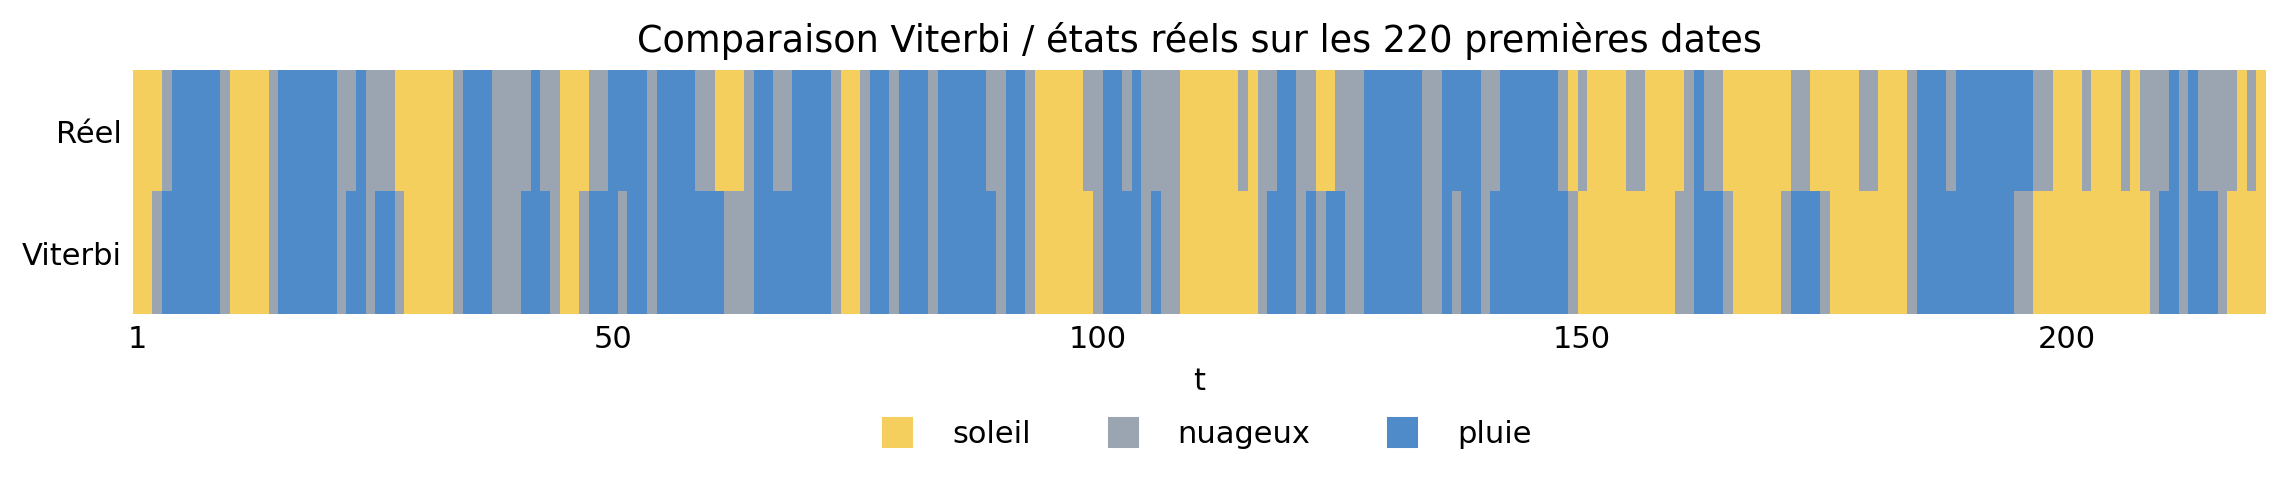
\includegraphics[width=0.90\linewidth]{Test/viterbi_vs_reel_220.png}

\vspace{0.2cm}


\caption{Comparison between the simulated true states and the Viterbi path over the first 220 dates.}
\end{figure}

Baum--Welch result: 
After running the Baum--Welch algorithm on the simulated data, we obtain the following estimated parameters.

The estimated transition matrix is
\[
\hat{A}
=
\begin{pmatrix}
0.7026 & 0.2956 & 0.0018 \\
0.2720 & 0.5963 & 0.1316 \\
0.1804 & 0.2172 & 0.6024
\end{pmatrix}.
\]

The estimated emission matrix is
\[
\hat{B}
=
\begin{pmatrix}
0.1070 & 0.8930 \\ 
0.5702 & 0.4298 \\
0.9895 & 0.0105 
\end{pmatrix}.
\]


\subsection{Interpretation of the Results Obtained on the Simulated Data}

\subsubsection{Analysis of the Forward Problem}

We apply the Forward criteria to the simulated trajectory. The evaluated model is the generating model
\(\lambda=(\pi,A,B)\).

\paragraph{Likelihood and Log-Likelihood}\mbox{}\\
\begin{table}[H]
\centering
\begin{tabular}{lr}
\toprule
Criterion & Value \\
\midrule
Series length \(T\) & 1001 \\
Number of free parameters \(p\) & 11 \\
Raw likelihood & \(1.3557\times 10^{-278}\) \\
Log-likelihood & -639.814329 \\
Average log-likelihood & -0.639175 \\
NLPD & 0.639175 \\
Indicative AIC & 1301.628658 \\
Indicative BIC & 1355.624961 \\
\bottomrule
\end{tabular}
\caption{Forward criteria on the complete series.}
\end{table}

The raw likelihood is very low, which is expected for a long observation sequence. We therefore use the log-likelihood
\[
\ell(\lambda)=\log P(Y_{1:T}\mid\lambda)=-639.814329.
\]
The average log-likelihood is
\[
\bar\ell(\lambda)=\frac{1}{T}\ell(\lambda)=-0.639175,
\]
and the negative log predictive density is
\[
\mathrm{NLPD}=-\bar\ell(\lambda)=0.639175.
\]

\begin{figure}[H]
\centering
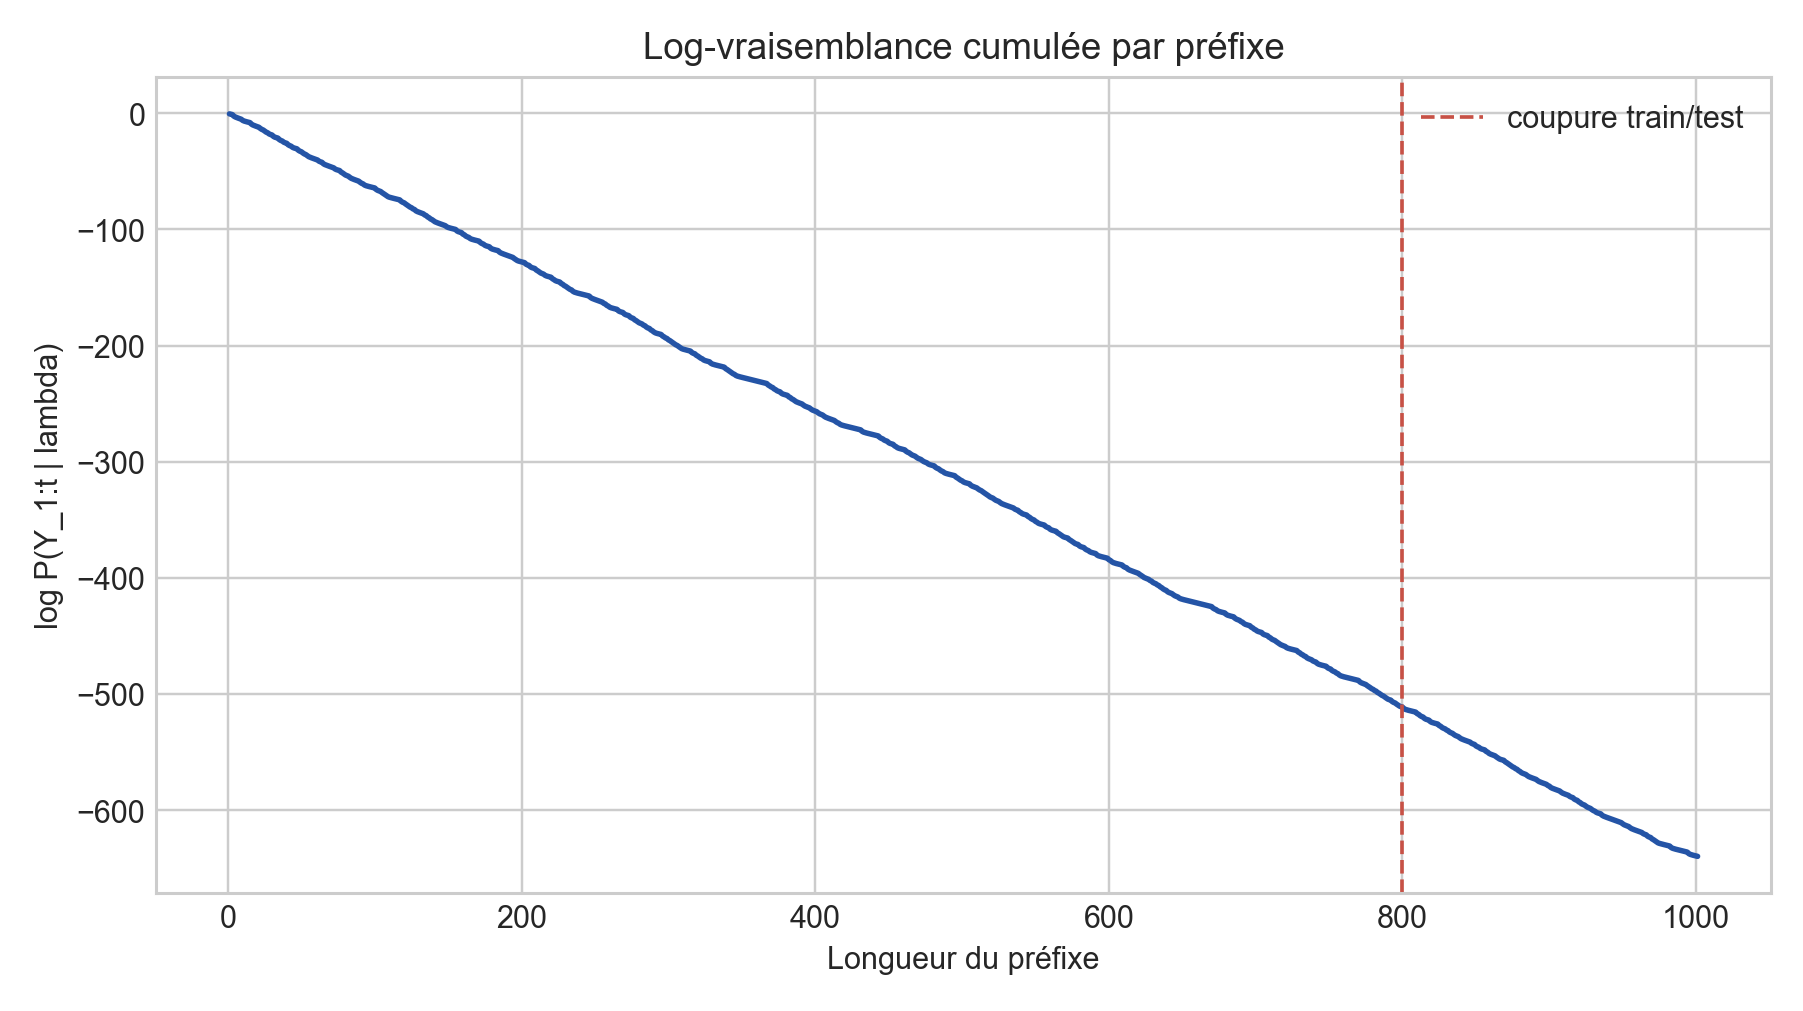
\includegraphics[width=0.82\linewidth]{Test/prefix_log_likelihood}
\caption{Cumulative log-likelihood by prefix.}
\end{figure}

\paragraph{Model Comparison}\mbox{}\\
We compare four models of the same dimension:
\[
\lambda_0=(\pi,A,B),
\qquad
\lambda_1=(\pi,A_{\mathrm{unif}},B),
\qquad
\lambda_2=(\pi,A,B_{\mathrm{unif}}),
\qquad
\lambda_3=(\pi_{\mathrm{unif}},A_{\mathrm{unif}},B_{\mathrm{unif}}).
\]
The model \(\lambda_1\) retains the emissions but makes the transitions uniform. The model
\(\lambda_2\) retains the transitions but makes the emissions uniform. The model \(\lambda_3\)
is entirely uniform.

For \(N=3\) states and \(M=2\) observations, we use
\[
p=(N-1)+N(N-1)+N(M-1)=11.
\]
The criteria are
\[
\mathrm{AIC}=-2\ell(\lambda)+2p,
\qquad
\mathrm{BIC}=-2\ell(\lambda)+p\log(T).
\]

\begin{table}[H]
\centering
\begin{tabular}{lrrrrr}
\toprule
Model & log-lik. & log-lik./obs. & NLPD & AIC & BIC \\
\midrule
Simulation model & -639.814329 & -0.639175 & 0.639175 & 1301.628658 & 1355.624961 \\
Uniform transitions & -689.395632 & -0.688707 & 0.688707 & 1400.791264 & 1454.787566 \\
Uniform emissions & -693.840328 & -0.693147 & 0.693147 & 1409.680655 & 1463.676958 \\
Uniform model & -693.840328 & -0.693147 & 0.693147 & 1409.680655 & 1463.676958 \\
\bottomrule
\end{tabular}
\caption{Forward comparison of the models.}
\end{table}

The simulation model minimises AIC and BIC. Models with uniform emissions obtain an average log-likelihood close to \(-\log(2)\), which indicates that removing the relationship between hidden states and observations strongly degrades Forward quality.

\begin{figure}[H]
\centering
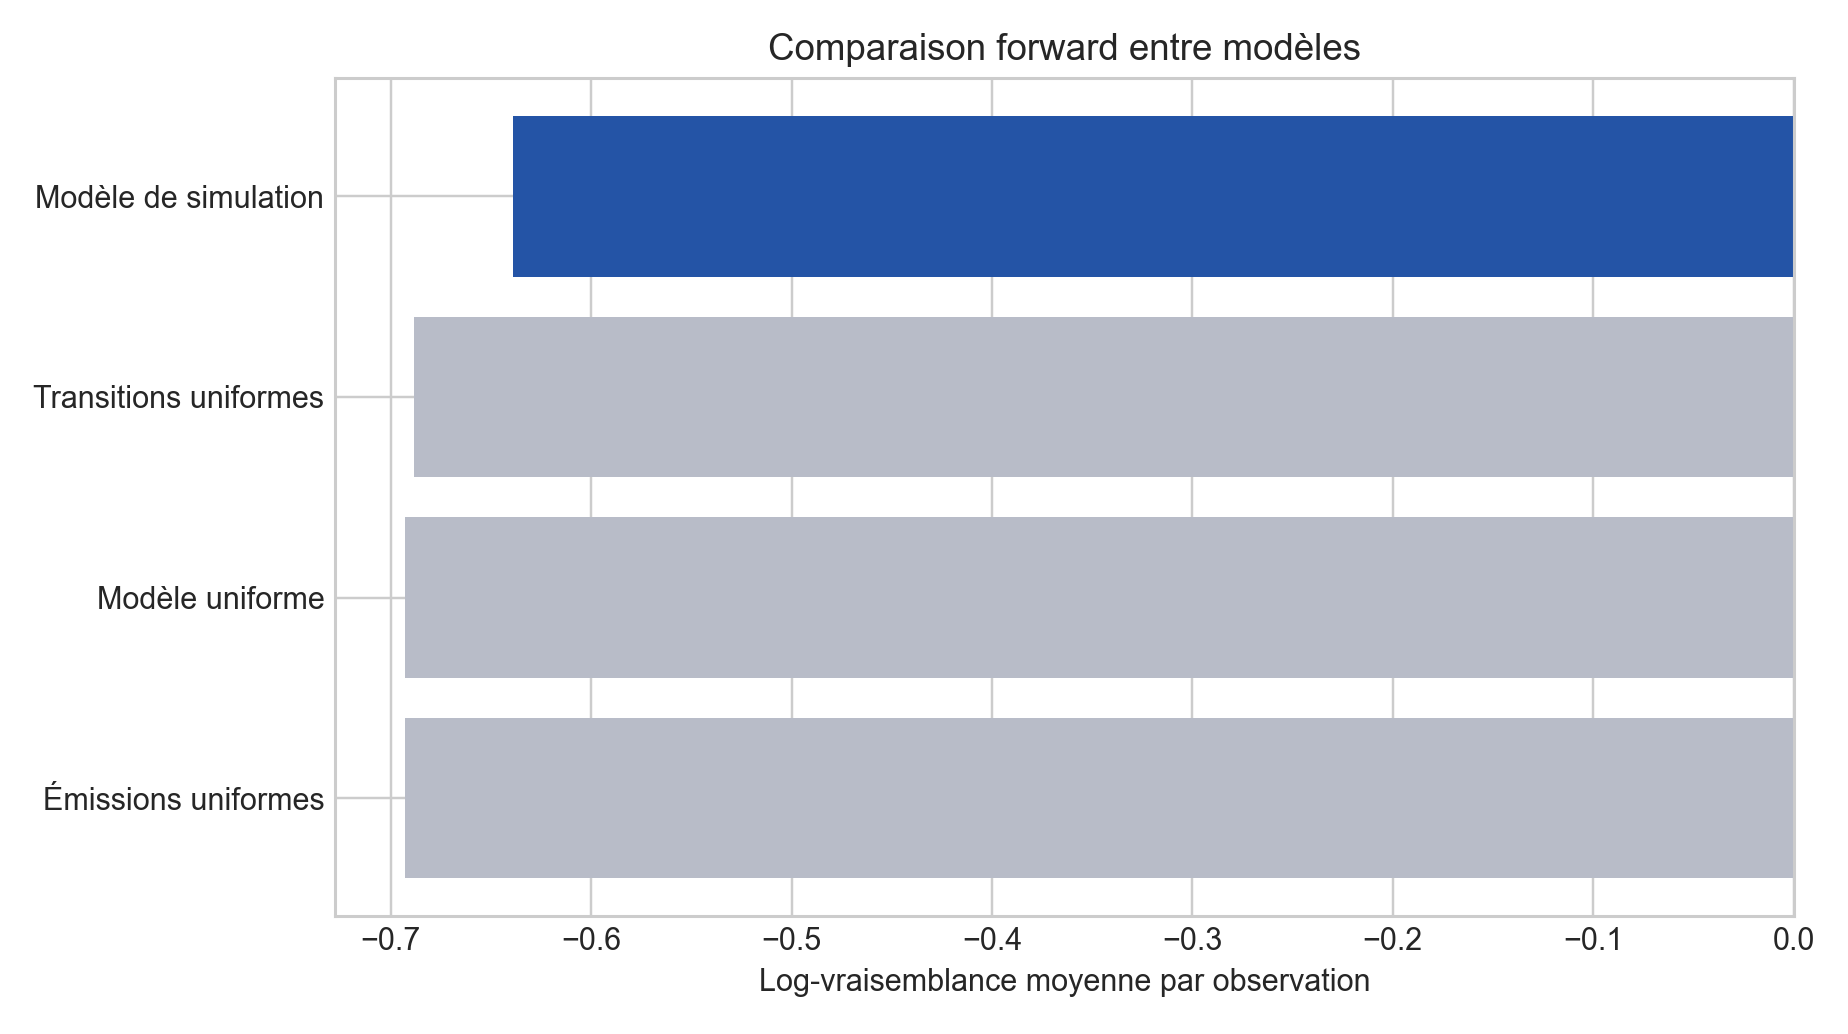
\includegraphics[width=0.82\linewidth]{Test/model_comparison}
\caption{Average log-likelihood by model.}
\end{figure}

\paragraph{Out-of-Sample Validation}\mbox{}\\
The series is split chronologically into 800 training observations and 201 test observations. Out-of-sample performance is measured by: 
\[
\ell_{\mathrm{test}}
=\log P(Y_{\mathrm{test}}\mid Y_{\mathrm{train}},\lambda),
\qquad
\mathrm{NLPD}_{\mathrm{test}}
=-\frac{1}{T_{\mathrm{test}}}\ell_{\mathrm{test}}.
\]

\begin{table}[H]
\centering
\begin{tabular}{lrrrr}
\toprule
Segment & \(T\) & log-lik. & log-lik./obs. & NLPD \\
\midrule
Training & 800 & -511.319586 & -0.639149 & 0.639149 \\
Conditional test & 201 & -128.494743 & -0.639277 & 0.639277 \\
Independent test & 201 & -128.462530 & -0.639117 & 0.639117 \\
\bottomrule
\end{tabular}
\caption{Out-of-sample Forward validation.}
\end{table}

The conditional test NLPD is 0.639277, very close to that obtained on the
training part. The model therefore retains stable predictive quality on the test observations.

\paragraph{Conclusion}\mbox{}\\
The Forward criteria provide a consistent evaluation: the average log-likelihood is -0.639175, the NLPD is 0.639175, the generating model minimises AIC and BIC among the models compared, and the out-of-sample NLPD remains close to that obtained over the training period.
The comparison with uniform models shows in particular that the emission matrix plays a central role: when the relationship between hidden states and observations is removed, the likelihood deteriorates substantially.

\subsubsection{Analysis of the Viterbi Problem}

We apply the criteria related to Viterbi decoding to the simulated trajectory. The path obtained is
denoted \(\hat X^V_{1:T}\).

\paragraph{Interpretation of the Detected Regimes}\mbox{}\\

We first examine whether the decoded states correspond to distinct observation profiles.

\begin{table}[H]
\centering
\begin{tabular}{lrrrr}
\toprule
Viterbi state & Dates & Observed umbrella & Theoretical umbrella & Observed no umbrella \\
\midrule
sunny & 408 & 9.56\% & 10.00\% & 90.44\% \\
cloudy & 206 & 12.62\% & 40.00\% & 87.38\% \\
rainy & 387 & 100.00\% & 90.00\% & 0.00\% \\
\bottomrule
\end{tabular}
\caption{Observation profile in each state decoded by Viterbi.}
\end{table}

The states \emph{sunny} and \emph{rainy} are well separated: the \emph{sunny} state is associated almost
always with \emph{No umbrella}, whereas the \emph{rainy} state is associated almost always with
\emph{Umbrella}. The \emph{cloudy} state is less clearly identified, which is consistent with
less extreme emission probabilities.

We then examine regime persistence.

\begin{table}[H]
\centering
\begin{tabular}{lrrrrr}
\toprule
Sequence & Changes & Rate & Runs & Mean length & Maximum length \\
\midrule
Viterbi & 326 & 32.60\% & 327 & 3.06 & 28 \\
Posterior decoding & 390 & 39.00\% & 391 & 2.56 & 21 \\
Local emission decoding & 358 & 35.80\% & 359 & 2.79 & 23 \\
\bottomrule
\end{tabular}
\caption{Persistence of the decoded sequences.}
\end{table}

The Viterbi path makes \(326\) changes, corresponding to a rate of \(32.60\%\). It is smoother than
posterior decoding, which corresponds to its objective: finding a coherent global trajectory.

\newpage

\paragraph{Comparison with Posterior Decoding and Local Decoding}\mbox{}\\

Posterior decoding chooses, at each date, the marginally most likely state:
\[
\hat X^P_t \in \arg\max_i P(X_t=i\mid Y_{1:T},\lambda).
\]
Local emission decoding chooses, at each date, the state that makes the current observation most likely:
\[
\widehat X_t^E=\arg\max_i b_i(Y_t).
\]
We compare the three decodings using the disagreement rate
\[
D_{VP}
=\frac{1}{T}\sum_{t=1}^T
\mathbf 1_{\{\hat X^V_t\neq \hat X^P_t\}}.
\]



\begin{table}[H]
\centering
\begin{tabular}{lr}
\toprule
Criterion & Value \\
\midrule
\(D_{VP}\) & 8.39\% \\
Viterbi vs local emission disagreement & 24.48\% \\
Mean posterior probability of the Viterbi state & 66.04\% \\
Median posterior probability of the Viterbi state & 67.99\% \\
Mean posterior margin & 38.33\% \\
Median posterior margin & 42.12\% \\
\bottomrule
\end{tabular}
\caption{Comparison between Viterbi and posterior decoding.}
\end{table}

We obtain \(D_{VP}=8.39\%\). The two methods therefore yield similar classifications. The
mean posterior probability of the state selected by Viterbi is \(66.04\%\), indicating that the
Viterbi path most often follows marginally plausible states.

\begin{figure}[H]
\centering
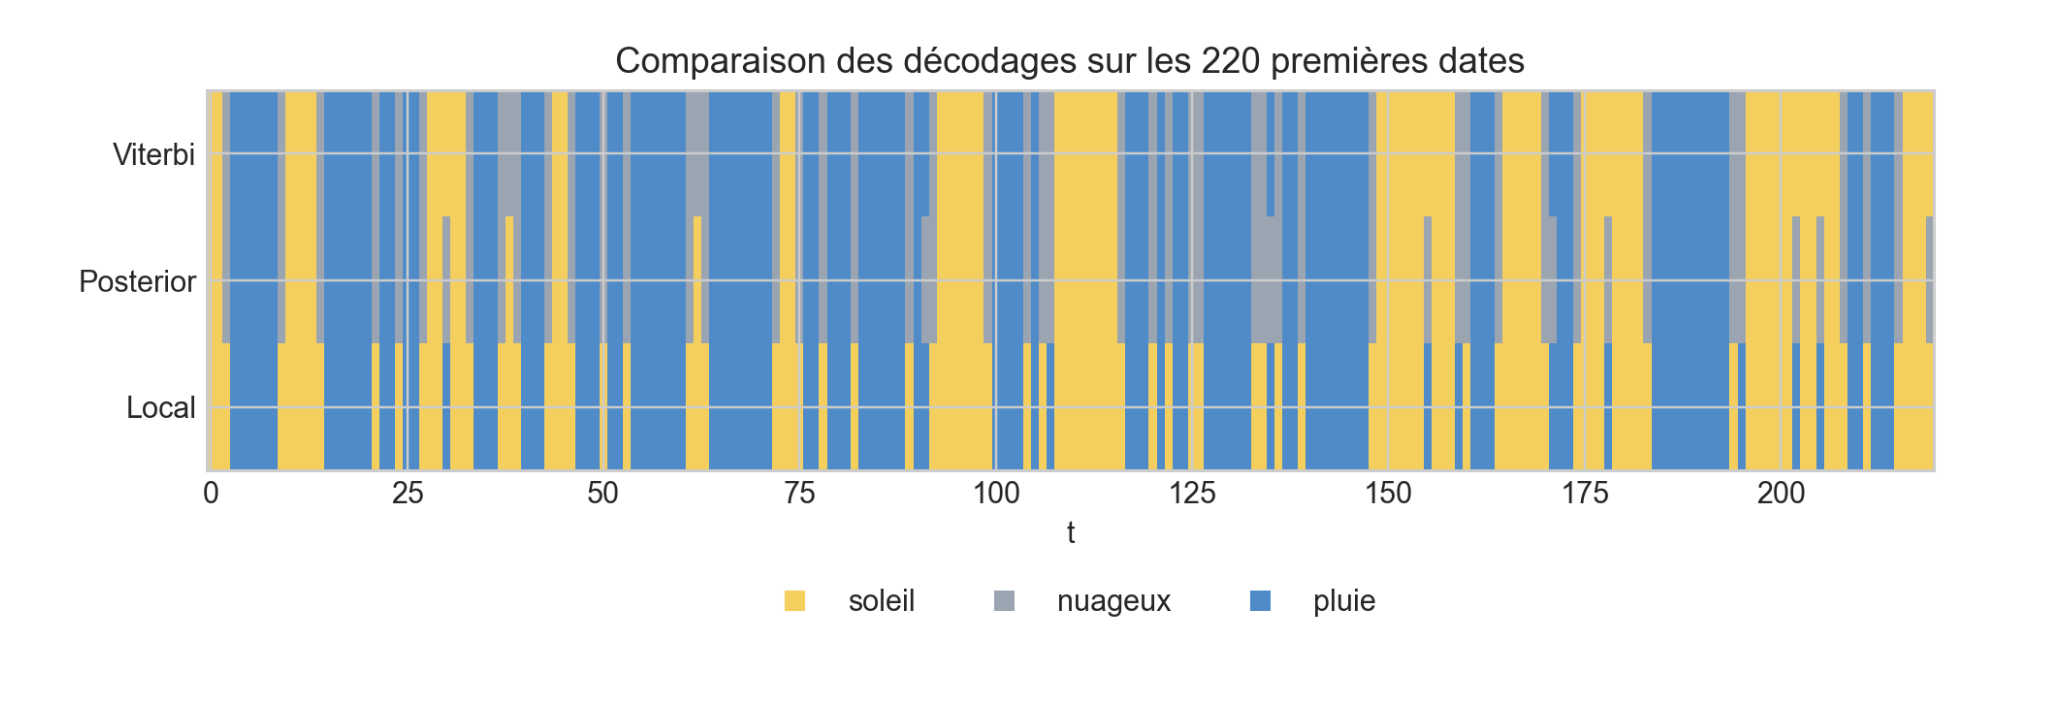
\includegraphics[width=0.90\linewidth]{Test/comparaison_visuelle_Viterbi}
\caption{Visual comparison between Viterbi, posterior decoding, and local decoding.}
\end{figure}

\paragraph{Conclusion}\mbox{}\\

The criteria provide a consistent interpretation of the decoding. The extreme regimes are readily
interpretable from the observations, and the disagreement rate with posterior decoding remains
low. The Viterbi path is also smoother than decodings based on local decisions.
The \emph{cloudy} regime remains less clearly separated, which is consistent with less discriminating
emission probabilities.

\subsubsection{Analysis of the Baum--Welch Problem}
We applied the Baum--Welch algorithm to the simulated dataset presented previously, running the estimation from several different initialisations. The objective here is to observe whether the estimated parameters are stable from one initialisation to another and whether the solutions obtained lead to comparable likelihoods.

Figure~\ref{fig:loglik_finales} compares the final log-likelihoods obtained for the different initialisations. The differences in log-likelihood per observation are very small, of order $10^{-4}$ to $10^{-3}$. This means that, from a likelihood perspective, the different estimates explain the observations in a rather similar manner. Some initialisations, in particular initialisations 9 and 10, give results that are almost identical to the best solution. Conversely, initialisation 8 has the largest difference, indicating a slightly inferior solution, although the difference remains small once scaled by the number of observations.

\begin{figure}[H]
    \centering
    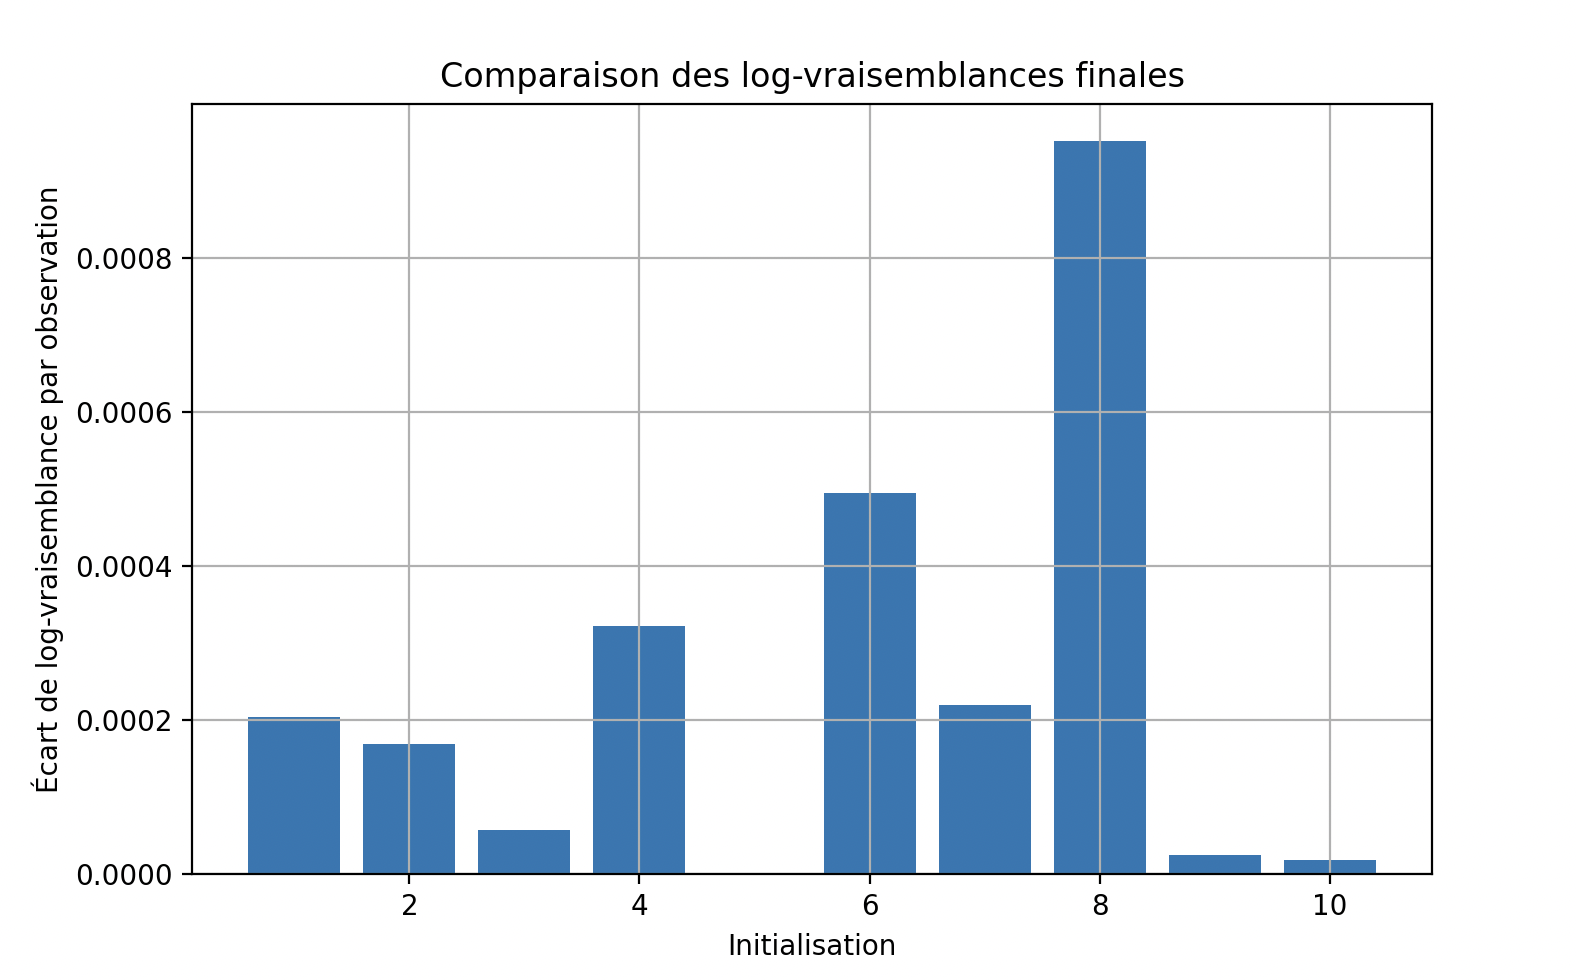
\includegraphics[width=0.85\textwidth]{Test/comparaison_log_vraisemblances.png}
    \caption{Comparison of final log-likelihoods according to initialisation.}
    \label{fig:loglik_finales}
\end{figure}

Figures~\ref{fig:stabilite_A} and~\ref{fig:stabilite_B} respectively show the stability of the transition matrix $A$ and the emission matrix $B$. These two matrices exhibit larger differences depending on the initialisation. In particular, initialisations 1, 2, 6, 7, and 8 lead to relatively large distances from the best solution. This shows that the estimated parameters are not perfectly stable.

This result is consistent with the expected behaviour of Baum--Welch: the algorithm may converge to different local maxima depending on the starting point. Thus, two initialisations may yield close final log-likelihoods while producing different matrices $A$ and $B$. In other words, likelihood alone is not always sufficient to guarantee that the estimated regimes have exactly the same interpretation.

\begin{figure}[H]
    \centering
    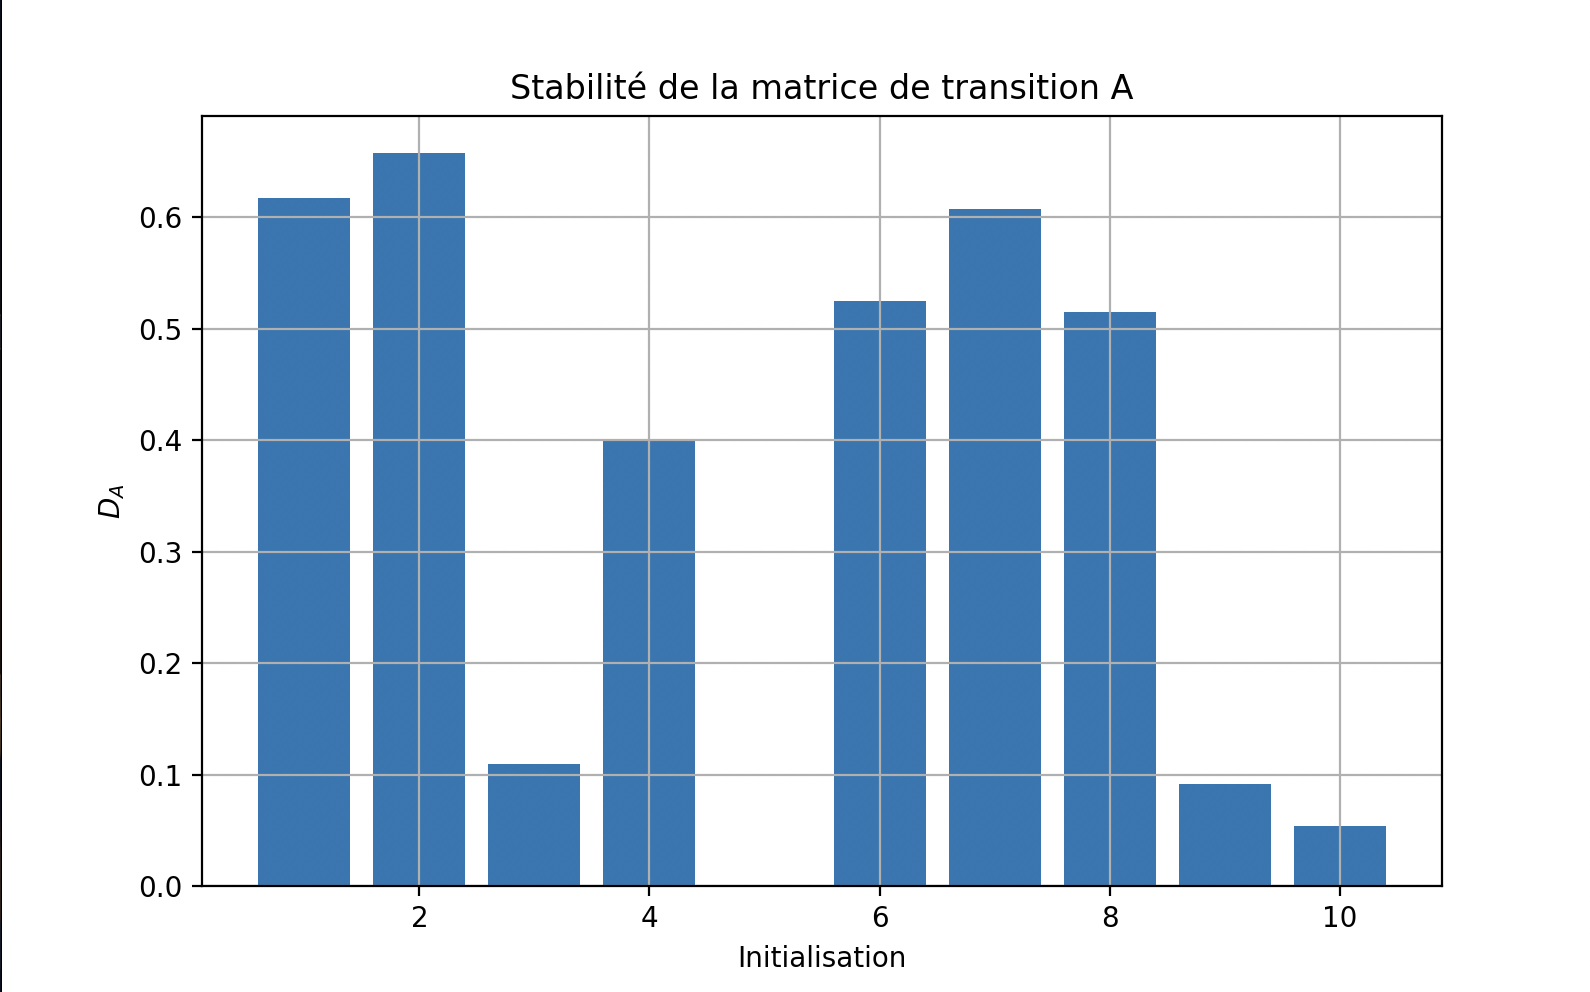
\includegraphics[width=0.85\textwidth]{Test/stabilite_A.png}
    \caption{Stability of the estimated transition matrix $A$.}
    \label{fig:stabilite_A}
\end{figure}

\begin{figure}[H]
    \centering
    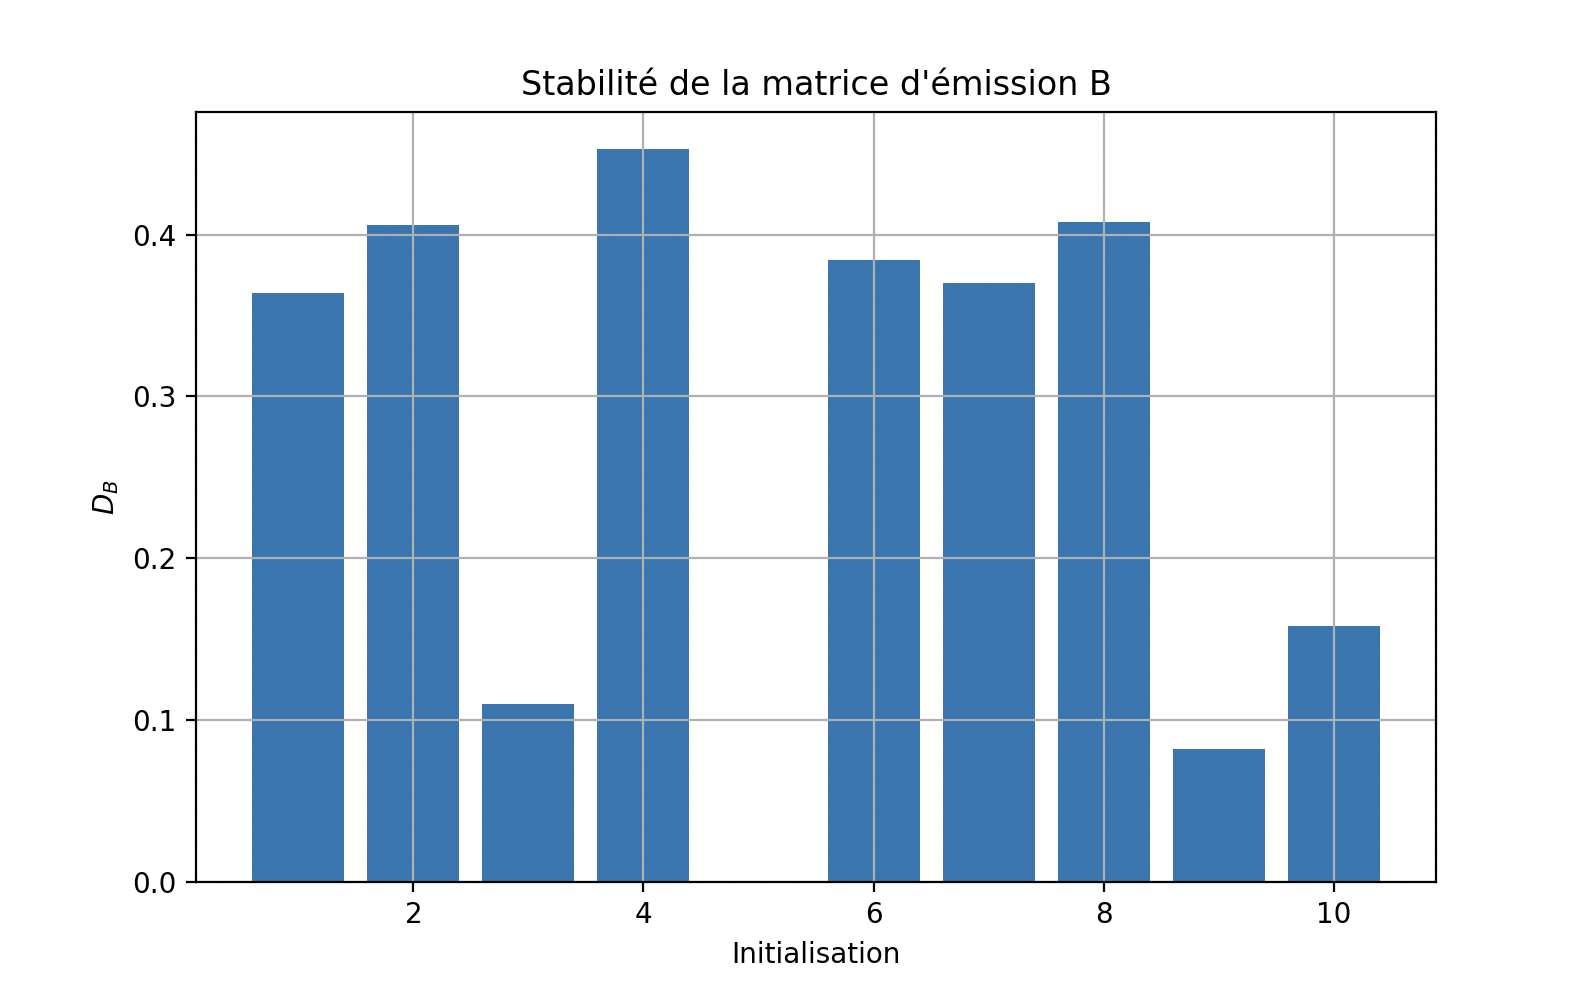
\includegraphics[width=0.85\textwidth]{Test/stabilite_b.png}
    \caption{Stability of the estimated emission matrix $B$.}
    \label{fig:stabilite_B}
\end{figure}

Figure~\ref{fig:stabilite_durees} makes it possible to interpret the stability of the transition matrix from a more concrete perspective by comparing average regime durations. We note that the initialisations for which the matrix $A$ is far from the reference are also those for which the average regime durations vary most strongly. Initialisations 1, 2, 6, 7, and 8 thus exhibit large differences, whereas initialisations 3, 9, and 10 are much closer to the reference solution.

This means that some estimates do not merely describe different matrices: they also lead to a different interpretation of the persistence of the hidden regimes. For example, a regime may be estimated as more stable or more transient depending on the initialisation. This observation is important because, in a hidden Markov model, the average time spent in each state is essential information for interpreting the regimes.

\begin{figure}[H]
    \centering
    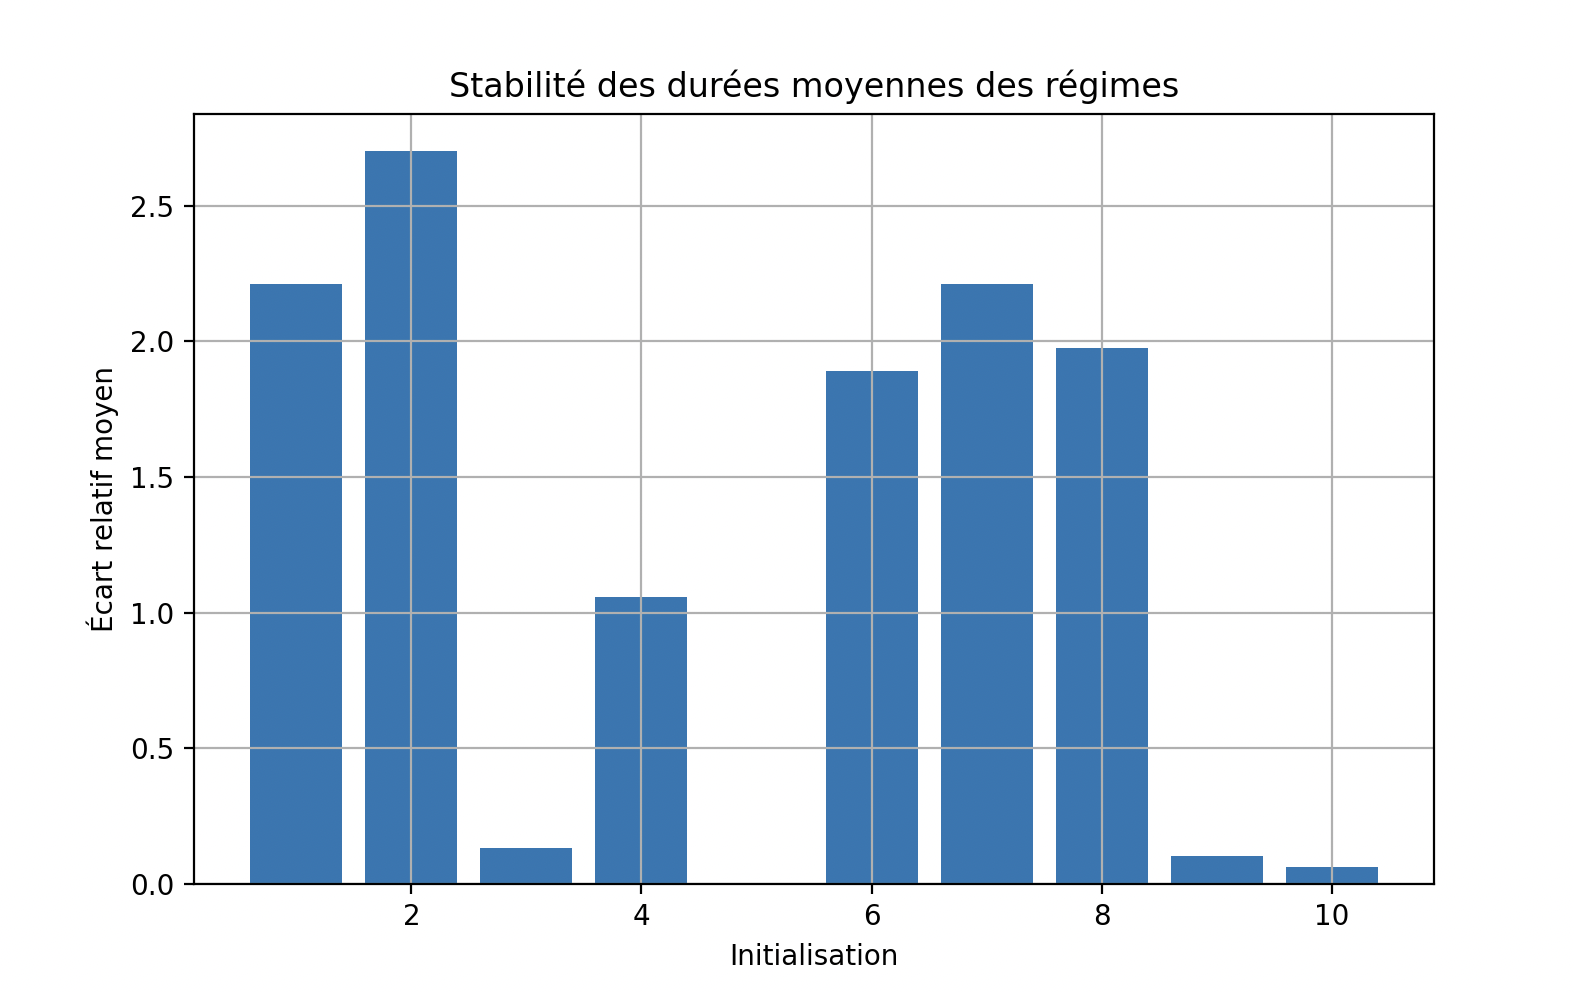
\includegraphics[width=0.85\textwidth]{Test/stabilite_durees.png}
    \caption{Stability of average regime durations.}
    \label{fig:stabilite_durees}
\end{figure}

Overall, the results show that the algorithm succeeds in obtaining solutions that are close in terms of likelihood, but that the estimated parameters may vary substantially depending on the initialisation. This difference is particularly visible for the transition matrix $A$, the emission matrix $B$, and the average regime durations. This confirms the relevance of running Baum--Welch several times with different initialisations, and then retaining the solution with the best final log-likelihood.

In our case, initialisations 9 and 10 appear very close to the reference solution, both in terms of likelihood and estimated parameters. Conversely, some initialisations yield parameters that are further away despite a relatively close final likelihood. We may therefore conclude that the algorithm performs correctly on the simulated data, but that its result remains sensitive to initialisation, which is a standard limitation of EM-type methods.



\subsection{Detection of Volatility Regimes on the VIX}


In this section, we apply a hidden Markov model to the VIX, i.e. the implied volatility index of the S\&P 500. The objective is to examine whether an HMM can automatically identify different market regimes from the evolution of volatility. Indeed, the VIX is often interpreted as an indicator of the level of stress or uncertainty in financial markets. A low VIX level generally corresponds to a calm period, whereas a high level is associated with periods of tension or crisis.

The data used are daily VIX observations between 2004 and 2024. After importing the data, we mainly retain the daily closing price of the VIX, denoted by $V_t$. In order to avoid constructing the model directly on the raw VIX level, we introduce several variables describing its dynamic behaviour. We first consider the logarithm of the VIX:
\[
    X_t = \log(V_t),
\]
then the daily log-return:
\[
    R_t = X_t - X_{t-1}.
\]
We also compute two measures of realised volatility, obtained as rolling standard deviations of the log-returns:
\[
    \sigma^{(20)}_t = \operatorname{std}(R_{t-19},\dots,R_t),
\]
and
\[
    \sigma^{(5)}_t = \operatorname{std}(R_{t-4},\dots,R_t).
\]
The first measure provides an estimate of realised volatility over approximately one trading month, whereas the second captures shorter and more reactive dynamics.

We therefore use the following vector as observed variables
\[
    Y_t =
    \begin{pmatrix}
        R_t \\
        \sigma^{(20)}_t \\
        \sigma^{(5)}_t
    \end{pmatrix}.
\]
These variables are then standardised before model estimation so that the different components have comparable orders of magnitude.

We consider a hidden Markov model with three hidden states:
\[
    S_t \in \{0,1,2\}.
\]
Conditionally on hidden state $S_t=i$, the observation $Y_t$ is assumed to follow a multivariate Gaussian distribution:
\[
    Y_t \mid S_t=i \sim \mathcal{N}(\mu_i,\Sigma_i),
\]
where $\mu_i$ is the mean vector associated with regime $i$ and $\Sigma_i$ is its covariance matrix. 

Model estimation is carried out using the Baum--Welch algorithm. Once the model has been estimated, the most likely sequence of hidden states is obtained using the Viterbi algorithm.

In our application, we selected three regimes in order to obtain a simple interpretation of market phases:
\[
    \text{calm regime}, \qquad
    \text{intermediate regime}, \qquad
    \text{crisis regime}.
\]
Since the states obtained by the HMM have no natural ordering, we then reorder them according to the average realised volatility $\sigma^{(20)}_t$. The regime with the lowest average volatility is called the calm regime, the one with intermediate average volatility is called the intermediate regime, and the one with the highest average volatility is called the crisis regime.
\vspace{0.5cm}

The average statistics obtained for the three regimes are as follows:
\[
\begin{array}{c|cccc}
\text{Regime} & \text{Average VIX} & \text{Average } R_t & \text{Average } \sigma^{(20)}_t & \text{Number of observations} \\
\hline
\text{Calm} & 16.3809 & 0.0007 & 0.0466 & 2364 \\
\text{Intermediate} & 20.0225 & -0.0021 & 0.0719 & 1751 \\
\text{Crisis} & 23.6703 & 0.0018 & 0.1134 & 1003
\end{array}
\]

\vspace{0.5cm}
The estimated transition matrix, after reordering the states, is given by:
\[
    \widehat{A}
    =
    \begin{pmatrix}
        0.972 & 0.020 & 0.007 \\
        0.038 & 0.941 & 0.021 \\
        0.000 & 0.053 & 0.947
    \end{pmatrix}.
\]
The diagonal coefficients are high. This means that the regimes are persistent.

The following figure represents the VIX over the period studied, with a background colour indicating the regime estimated by the HMM.

\begin{figure}[h]
    \centering
    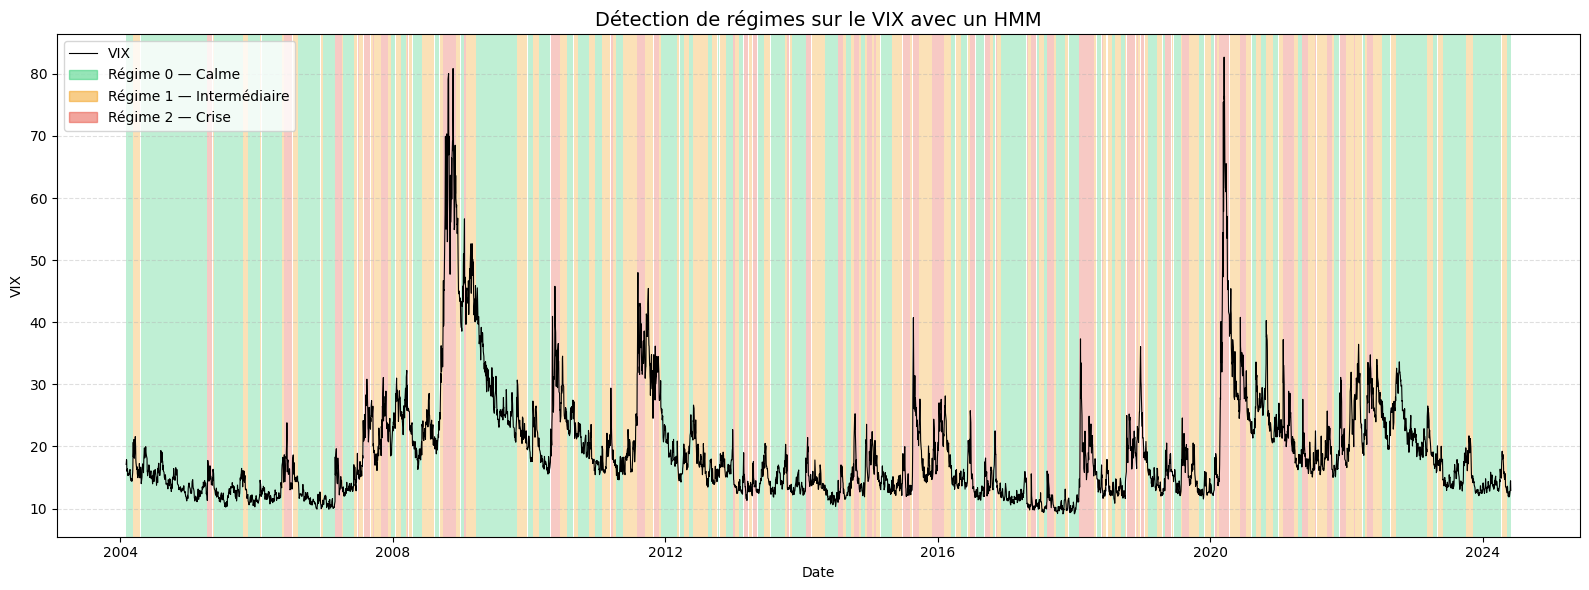
\includegraphics[width = 1\textwidth]{Figures/regime_detectionVIX.png}
    \caption{Regime detection on the VIX index between 2004 and 2024}
    \label{fig:mon_image}
\end{figure}

We observe that the model mainly identifies calm phases, associated with the lowest-volatility regime, while switching to the intermediate and crisis regimes during episodes of high instability. These changes appear in particular around major increases in the VIX, such as during the 2008 financial crisis, the sovereign debt crisis in 2011--2012, and the volatility shock observed in 2020. The model therefore appears capable of automatically identifying periods of market stress from the variables constructed using the VIX.

It should nevertheless be emphasised that the estimated regimes do not directly have an economic interpretation. The HMM classifies observations according to their statistical properties, in particular returns and realised volatility levels, but it does not itself associate a hidden state with a specific economic event. The interpretation of the regimes must therefore be performed a posteriori by comparing the detected periods with known episodes of market tension.

The results also depend on the modelling choices, in particular the variables used, the number of hidden states, and the initialisation of the algorithm. The choice of three regimes provides a natural interpretation here, but other specifications could lead to a different segmentation.

This application thus illustrates the relevance of hidden Markov models for the analysis of financial series. In the case of the VIX, the HMM provides a simple probabilistic method for classifying market periods according to their volatility level and persistence dynamics.

\subsection{Analysis of the Quality of the Baum--Welch Estimation on the VIX}

We apply the Baum--Welch evaluation criteria to the HMM estimated on the VIX. The observations used are the same as previously:
\[
Y_t =
\begin{pmatrix}
R_t \\
\sigma_t^{(20)} \\
\sigma_t^{(5)}
\end{pmatrix},
\]
where \(R_t\) is the daily log-return of the VIX, \(\sigma_t^{(20)}\) is the realised volatility over twenty days, and \(\sigma_t^{(5)}\) is the realised volatility over five days. The variables are standardised before estimation. The model has three hidden states and multivariate Gaussian emissions.

The series used contains \(5118\) observations, from 2 February 2004 to 31 May 2024.

\paragraph{Log-Likelihood Convergence}\mbox{}\\

Baum--Welch is run with several initialisations. The best solution is obtained at the tenth initialisation. The final log-likelihood is
\[
\ell(\widehat{\lambda})=-14300.087178,
\]
corresponding to an average log-likelihood of
\[
\frac{\ell(\widehat{\lambda})}{T}=-2.794077.
\]

\begin{table}[H]
\centering
\begin{tabular}{lr}
\toprule
Criterion & Value \\
\midrule
Number of observations \(T\) & 5118 \\
Best initialisation & 10 \\
Number of iterations & 36 \\
Final log-likelihood & -14300.087178 \\
Average log-likelihood & -2.794077 \\
Final gain per observation & \(9.728857\times 10^{-11}\) \\
Final relative gain & \(3.481714\times 10^{-11}\) \\
Number of detected decreases & 0 \\
\bottomrule
\end{tabular}
\caption{Convergence of Baum--Welch on the VIX.}
\end{table}

The log-likelihood is increasing and no numerical decrease is detected. The final gain per observation is far below \(10^{-6}\), which indicates that the algorithm has stabilised. The convergence is therefore satisfactory.

\paragraph{Stability of the Estimated Parameters}\mbox{}\\

Since Baum--Welch depends on the initialisation, the estimation is repeated ten times. The states are then aligned in order to correct for label switching. For the emissions, the discrete criterion \(D_B\) is replaced by a Gaussian distance based on a symmetrised Kullback--Leibler divergence between the emission distributions.

\begin{table}[H]
\centering
\begin{tabular}{lr}
\toprule
Stability criterion & Average value \\
\midrule
\(D_\pi\) & \(2.563015\times 10^{-109}\) \\
\(D_A\) & \(5.050970\times 10^{-7}\) \\
Gaussian \(D_B\) & \(7.307790\times 10^{-10}\) \\
Mean relative duration difference & \(1.257620\times 10^{-5}\) \\
Maximum log-likelihood difference per observation & \(1.587589\times 10^{-10}\) \\
\bottomrule
\end{tabular}
\caption{Stability of the Estimates according to Initialisation.}
\end{table}

\begin{figure}[H]
\centering
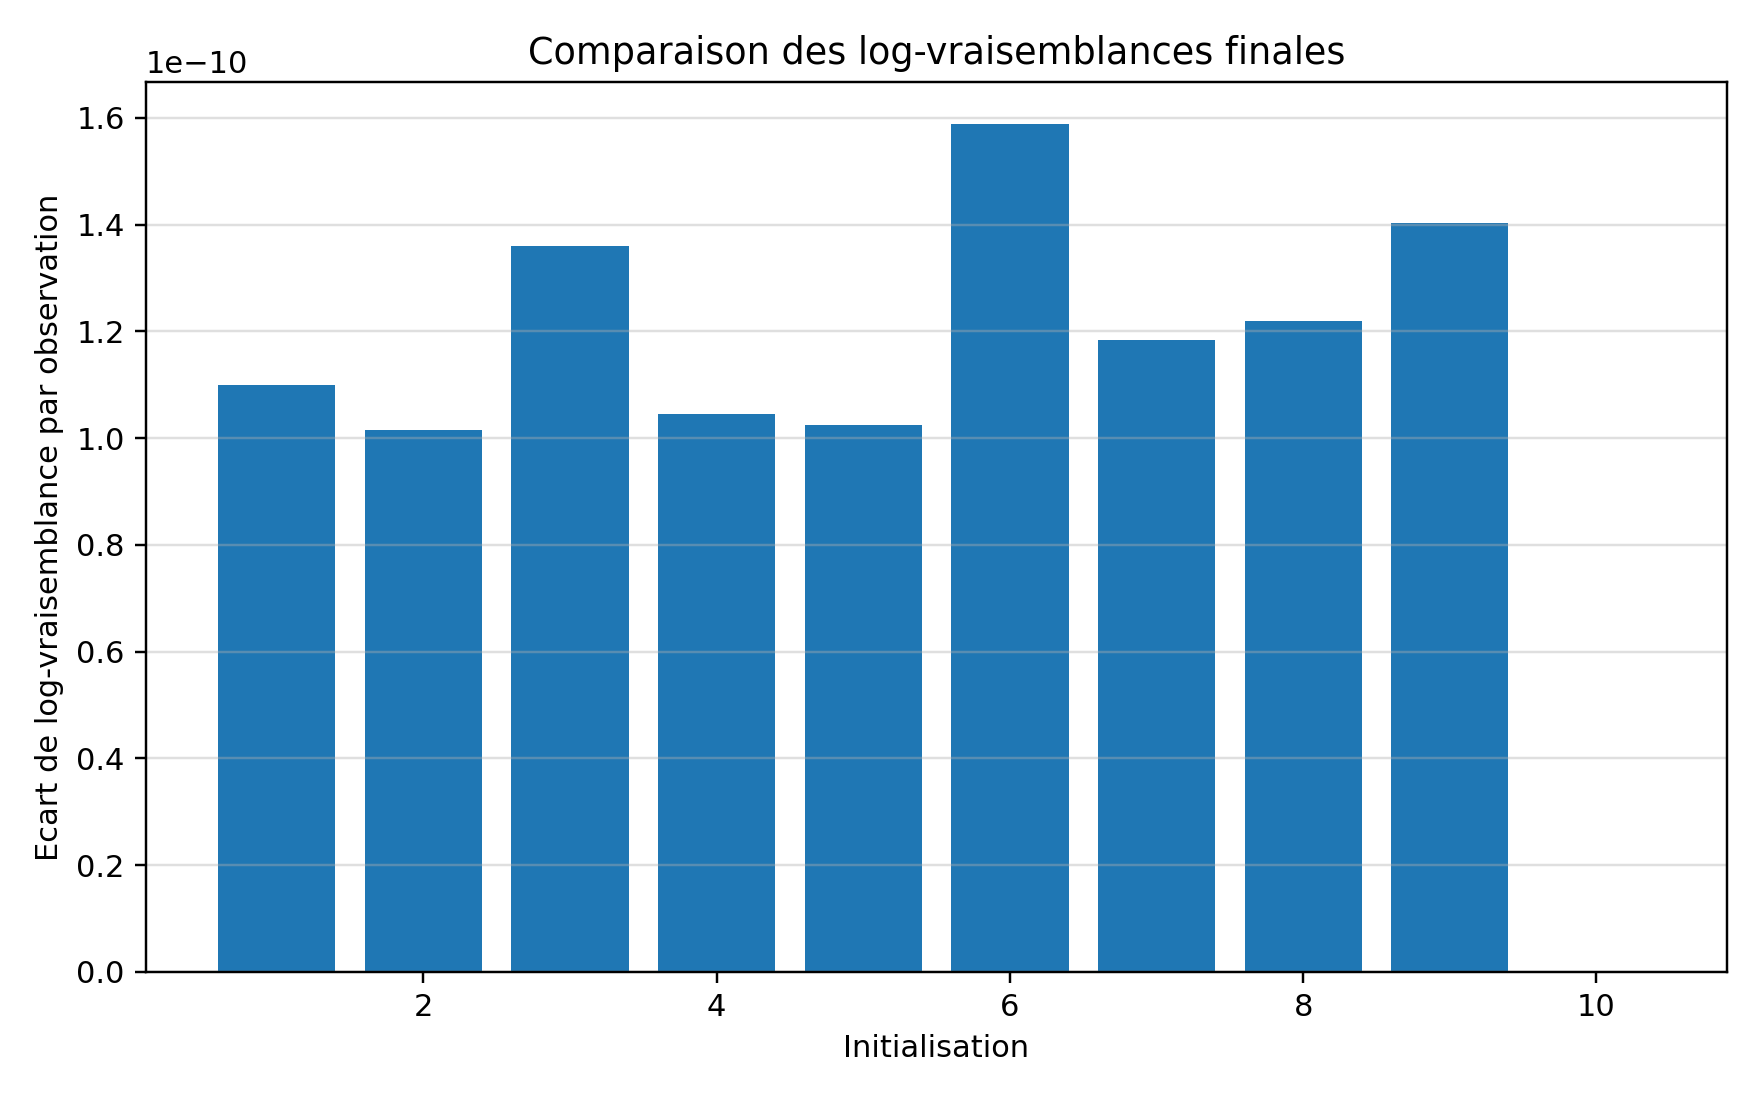
\includegraphics[width=0.82\linewidth]{Test/comparaison_log_vraisemblances_vix.png}
\caption{Comparison of final log-likelihoods.}
\end{figure}

The differences between initialisations are extremely small. The final log-likelihoods are almost identical, the transition matrices are very close, and the Gaussian emissions remain stable after state alignment. Unlike the case in which Baum--Welch converges to several distinct local optima, the results obtained here indicate a very stable solution for this choice of variables and number of states.

\paragraph{Out-of-Sample Validation}\mbox{}\\

The series is split chronologically: \(4094\) observations are used for training and \(1024\) observations are used for testing. The model is estimated on the training period and then evaluated on the subsequent period.

\begin{table}[H]
\centering
\begin{tabular}{lrrr}
\toprule
Segment & \(T\) & Log-likelihood & NLPD \\
\midrule
Training & 4094 & -11536.441391 & 2.817890 \\
Conditional test & 1024 & -2774.008272 & 2.708992 \\
Independent test & 1024 & -2782.320895 & 2.717110 \\
\bottomrule
\end{tabular}
\caption{Out-of-sample validation of the HMM on the VIX.}
\end{table}

The conditional test NLPD is \(2.708992\), compared with \(2.817890\) over the training period. Thus, the model does not exhibit out-of-sample deterioration on this chronological split. This comparison does not mean that the test period is always easier to predict, but it indicates that the parameters estimated on the first part of the series retain a good ability to assign high density to future observations.

\paragraph{Conclusion}\mbox{}\\

The criteria applied to the VIX provide a favourable evaluation of the Baum--Welch estimation. The log-likelihood converges without any numerical decrease, the different initialisations lead to virtually the same solution after state alignment, and the resulting regimes are interpretable in terms of market volatility. Out-of-sample validation confirms that the model remains stable over the test period. The main difference from the simulation is that there are no observable true hidden states here: the evaluation therefore relies on convergence, parameter stability, the economic consistency of the regimes, and predictive performance.

\section{References}

\begin{thebibliography}{99}

\bibitem{rabiner1989}
Rabiner, L. R. (1989).
\emph{A tutorial on hidden Markov models and selected applications in speech recognition}.
\url{https://www.cs.ubc.ca/~murphyk/Bayes/rabiner.pdf}
\bibitem{jurafsky2026}
Jurafsky, D., \& Martin, J. H. (2026).
\emph{Hidden Markov Models}.
In \emph{Speech and Language Processing} (Chapter A, draft of January 6, 2026).
Stanford University.
\url{https://web.stanford.edu/~jurafsky/slp3/A.pdf}

\bibitem{sublime2022}
Sublime, J. (2022).
\emph{Data Analysis -- Lecture 9: Time series analysis, Hidden Markov Models}.
Engineering school lecture notes, France.
HAL, hal-03845332.
\url{https://hal.science/hal-03845332/document}

\bibitem{baum1966}
Baum, L. E., \& Petrie, T. (1966).
\emph{Statistical inference for probabilistic functions of finite state Markov chains}.
The Annals of Mathematical Statistics, 37(6), 1554--1563.
\url{https://doi.org/10.1214/aoms/1177699147}

\bibitem{baum1970}
Baum, L. E., Petrie, T., Soules, G., \& Weiss, N. (1970).
\emph{A maximization technique occurring in the statistical analysis of probabilistic functions of Markov chains}.
The Annals of Mathematical Statistics, 41(1), 164--171.
\url{https://doi.org/10.1214/aoms/1177697196}


\bibitem{wu1983}
Wu, C. F. J. (1983).
\emph{On the convergence properties of the EM algorithm}.
The Annals of Statistics, 11(1), 95--103.
\url{https://doi.org/10.1214/aos/1176346060}


\bibitem{leroux1992}
Leroux, B. G. (1992).
\emph{Maximum-likelihood estimation for hidden Markov models}.
Stochastic Processes and their Applications, 40(1), 127--143.
\url{https://doi.org/10.1016/0304-4149(92)90141-C}


\bibitem{lember2014}
Lember, J., \& Koloydenko, A. A. (2014).
\emph{Bridging Viterbi and posterior decoding: A generalized risk approach to hidden path inference based on hidden Markov models}.
Journal of Machine Learning Research, 15, 1--58.
\url{https://jmlr.org/papers/v15/lember14a.html}

\bibitem{akaike1974springer}
Akaike, H. (1974).
\emph{A New Look at the Statistical Model Identification}.
In E. Parzen, K. Tanabe, \& G. Kitagawa (Eds.),
\emph{Selected Papers of Hirotugu Akaike}
(pp. 215--222).
Springer Series in Statistics. Springer, New York, NY.
\url{https://doi.org/10.1109/TAC.1974.1100705}


\end{thebibliography}




\end{document}